%%%%%%%%%%%%%%%%%%%%%%%%%%%%%%%%%%%%%%%%%%%%%%%%%%%%%%%%
% Written by: Erick Cobos Tandazo (a01184587@itesm.mx)
% Date: 7-April-2014
%
% Project proposal for my Master's thesis
%%%%%%%%%%%%%%%%%%%%%%%%%%%%%%%%%%%%%%%%%%%%%%%%%%%%%%%%%

\documentclass[11pt]{article}

% Packages
\usepackage[utf8]{inputenc}	% Spanish accents
\usepackage{proposalEMCT} 	% Title pages and overall format
\usepackage{verbatim} 		% Block Comm\usepackage{textcomp}ents
\usepackage{textcomp}		% For the degree sign(°)
\usepackage{hyperref}		% To manage \url and citations as links to the reference part.
\usepackage{subcaption}		% For subfigure in breastcancer.tex
\usepackage{amssymb}		% For R (real numbers) symbol, among others.
\usepackage{amsmath}		% Add text to math and further math equations.

% Set properties of the document
\propautor{Erick Michael Cobos Tandazo}	% Author name
\propautormat{1184587}			% Author ID number
\propmes{May 14}			% Date (month)
\propanio{2015}				% Year
\propcd{Monterrey, N.L.}		% Place
\proptitulo{Early Detection and Diagnosis of Breast Cancer Lesions in Digital Mammograms using Deep Convolutional Networks}	% Title
\propasesor{Dr.~Hugo Terashima Mar\'{i}n}	% Advisor
\propsinodalA{Por definir}		% First supervisor
\propsinodalB{Por definir}		% Second supervisor.
\propdirectorPG{Dr.~Ram\'{o}n Brena Pinero}	% Program Director
\propPG{Engineering and Sciences}		% School/Department
\propcampus{Monterrey}			% University Campus
\propgrado{Master of Science}		% Academic degree
\propgradosiglas{M.Sc.}			% Academic degree abbreviation
\propespecialidad{Intelligent Systems}	% Subject
%%%%%%%%%%%%%%%%%%%%%%%%%%%%%%%%%%%%%%%%%%%%%%%%%%%%%%%%%%%%%%%%%%%%%%%%%%%%%



\begin{document}

\propportada                        % Genera la portada.
\proppagfirmas                      % Genera la pagina de firmas.
\thispagestyle{empty}
\tableofcontents                    % Genera indice general.
\newpage
\sloppy
\newpage
\pagenumbering{arabic}

\begin{abstract}
Breast cancer is one of the most common and deadliest cancer in woman around the world. The best tools used today for early breast cancer diagnosis are screening mammograms; mammograms are x-ray pictures of the breast used by radiologists to identify microcalcifications and breast masses, signs of early breast cancer development. Traditional computer systems use handmade features and complex image techniques to detect these lesions in mammographic images. In this work, we plan to use convolutional networks, a recent development in computer vision, which can automatically learn the relevant features for the classification task given enough training data. Convolutional networks have been used in some studies for breast cancer detection but we hope to introduce newer features and carefully tune the architecture to produce improved results. Additionally, this will be the first approximation to use deep learning techniques as part of an ongoing project in the institution which aims to develop a computer-aided diagnosis system for breast cancer. This thesis proposal is presented for approval to obtain the degree of Master of Science in Intelligent Systems.
%Keywords: convolutional neural  networks, breast cancer, CAD, mammograms
\end{abstract}

\section{Introduction}
\begin{comment} 
Hook(first paragarpah) : Automatic breast cancer diagnosis is a very difficult taks for current automatic computationnal systems. In this article,  we apply deep learning techniques to digital mammogrpahic images and obtain better results than presented to date. We show or prove or use this technique to obtain this... (when we have results)
Automatic breast cancer diagnosis is a very difficult task for current computational systems. In this thesis, we apply deep learning techniques to digital mammographic images in order to improve the performance of such systems. We layout here the hypotheses, experiments and goals of our future research.
\end{comment}
Accurately diagnosing breast cancer is hard for current computational systems; in this thesis, we use deep learning to improve their performance.

Breast cancer is caused by abnormal cells that grow out of control forming tumors and invading surrounding breast tissue.
%If this growth is not controlled it can cause serious illness or death.
It has the highest incidence rate of any cancer in the United States, an estimated 14.1\% of cancer diagnoses in 2015, and the third highest mortality accounting for 6.9\% of all cancer-related deaths. Among women, it is the most commonly diagnosed cancer (28.6\%) and has the highest death rate (14.5\%) besides lung cancer~\cite{ACS2015}. The American Cancer Society recommends that women aged 45 or older should get mammograms, images of the breast which show signs of tumor formation, annually or biennially~\cite{Oeffinger2015}. We consider two of the lessions that can be found on a mammogram: clustered microcalcifications, tiny deposits of calcium that could appear around cancerous tissue; and breast masses, more direct signs of the existence of a tumor although often benign.
%For the diagnosis of suspicious areas, more mamograms or a biopsy are normally required. The quality of a mmamogram and the diligence and experience of the radiologist is an important factor to succesfully detect breast cancer.

We focus on using mammograms to automatically detect these lesions and predict the probability of breast cancer on the patient. Although manual examination of mammograms has a high sensitivity rate, automatic examination could be used by radiologists as a second informed opinion or as a help in deciding which regions should be further analysed. It could also be used where doctors are unavailable. With this motivation, the department created a project to design a computer-aided diagnosis system (CAD) for breast cancer. This thesis falls under the scope of this project as the first attempt to use deep learning for breast cancer diagnosis.

Traditional CAD systems for breast cancer work as a pipeline where each stage uses different computer vision and machine learning techniques. An standard pipeline will, for instance, preprocess the image, identify and segment the relevant parts of the picture, extract features from the segmented parts and train a classifier on the extracted features. Although some successful systems are built in this manner, they have a few disadvantages: each stage is a separate component and hence each of them needs to be improved to notably improve overall results, it is composed of dependent stages so that changes on one component affect the performance of other parts of the system, it uses complex image vision techniques that are difficult to handcraft to segment the images and extract features, it requires expert knowledge to be properly tuned, among others.

We plan to investigate the potential of convolutional networks to replace some if not all of the stages of traditional image processing systems. Convolutional networks~\cite{Fukushima1980,LeCun1998}, a natural extension to feedforward neural networks, are a statistical learning classifier that uses raw images as input and learns the important features for the classification task as it is trained. Convolutional networks work well with minimally preprocessed images, can be trained to be rotational and translational invariant and perform segmentation, feature extraction and classification in one step. In our case, convolutional networks simplify classification potentially reducing it to a single component that we can train from labelled data and tune to obtain better results. Although convolutional networks have some drawbacks, they are the state-of-the-art technology for object recognition~\cite{Russakovsky2014} and we believe it is worthy to experiment with them.

%Summary of the related work part here(this guys dd it first and this guys and i'm gteting my ideas from here and there and my contribution is this...)
Researchers have used small convolutional networks to detect breast masses from normal tissue~\cite{Sahiner1996} and individual microcalcifications from noise in the image~\cite{Lo1995, Ge2007}. In these experiments mammograms were preprocessed, enhanced and potential masses and microcalcifications were segmented and presented to the network for classification. We plan to use the available data and aggresively augment it using rotations, translations and reflections so that we could train bigger networks that would potentially learn more complex features. Furthermore, we plan to apply some of the most recent advances such as rectified linear unit activations, max-pooling, dropout, etc. to new tasks related to breast cancer detection where they have not yet been applied. For instance, the detection and diagnosis of masses and clustered microcalcifications.

We start our experiments by training a simple convolutional network to detect masses and clustered microcalcifications, later we train a more complex network architecture including some of the most recent advances and finally use the gathered knowledge to build an optimal convolutional network with tuned hyperparameter. As further experiments and depending on the available time we plan to pretrain a convolutional network with a different image database and fine-tune it using our database, use an all convolutional architecture, account for the problem of using an unbalanced data set and use an ensemble of networks. We intend to learn whether convolutional networks can automatically detect and diagnose breast cancer lesions, what are the advantages of using more data, a bigger architecture and tuned hyperparameters and whether we can achieve results similar to those of traditional systems.

This document offers an insight into the problem with traditional methods for image analysis in Section~\ref{sec:ProblemDefinition}. It exposes the particular objectives and hypotheses of the thesis in Sections~\ref{sec:Objectives} and~\ref{sec:Hypothesis}. Section~\ref{sec:Background} presents a comprehensive background of the scientific concepts used throughout the document and lastly a detailed methodology and work plan are shown in Sections~\ref{sec:Methodology} and~\ref{sec:WorkPlan}.

\begin{comment}
En esta sección se espera que el autor describa en forma más amplia a como
se presentó en el {\it Resumen}, algunos aspectos como el contexto de la
investigación, el problema a resolver, la forma propuesta de resolver, algunos
antecedentes, entre otros.

Los puntos importantes en la {\it Introducción} son:
\begin{itemize}
	\item Introducción al contexto donde se va a realizar la propuesta
	\item Determinar la situación problemática 
	\item Definir el problema y los factores y aspectos más importantes que intervienen  en el problema
	\item Justificar por qué es importante resolver ese problema
 Michael: Hasta aqui es pareciod a lo de definicion de problema. M
	\item Explicar lo qué se ha hecho para resolver ese problema
	\item Describir el modelo de solución del problema
	\item Establecer los posibles logros en la solución del problema
	\item Describir la organización del documento
\end{itemize}

{\bf Ejemplo de Cita Bibliográfica:}

En años recientes se ha manifestado interés en el área de Algoritmos Genéticos
con la Teoría de Dificultad
Walsh polynomials \cite{Clear2}....... \\


{\bf No olviden incluir en donde corresponde
 la motivación, la justificación, el alcance de la
investigación, los recursos y las suposiciones...}
\end{comment}


\section{Problem Statement and Motivation}
\label{sec:ProblemDefinition}
%[[Image] segmentation [is the process of|is the task of] partitions [an|the] image into [multiple [disjoint]|disjoint] regions[, essentially [labelling each pixel as belonging to a class from a predefined set of classes|assigning a [class|label] to each pixel. [in the image]]  |Partitioning an image into multiple regions is called image segmentation.][[[In machine learning,] this reduces to|This is equivalent to| similarly,] [classifying|assigning] each pixel [into|as part of| as belonging to|to] a [class from a] given set of classes]] For instance, each pixel in a street image could be classified as [part of a] road, building, tree, pedestrian or bicycle.
Image segmentation partitions an image into multiple regions, essentially assigning a class to every pixel in the image; for instance, classifying each pixel in a street image as road, building, sky, tree, car, pedestrian, bycicle or background. Lesion segmentation is tasked with separating lesions from normal tissue in medical images. When searching for abnormal findings, radiologists perform lesion segmentation---although implicitly. Traditional CAD systems for lesion segmentation are based on computer vision methods that are often convoluted and hard-to-adapt~\footnote{See~\cite{Ashraf2013} for an example.}. 

Despite their widespread use and relative success, various limitations should be address to further advance the field:
\begin{itemize}
	\item Lack of standard preprocessing techniques. Some techniques are commonly used but their performance can vary.
	\item Handcrafted features. The features extracted from the image are chosen beforehand (maybe designed with the help of experts) and special filters and image techniques are used to extract them.
	\item Expertise needs. They require knowledge in various fields such as radiology, oncology, image processing, computer vision, machine learning, etc.
	\item Pipeline structure. Systems are composed of many sequential steps. At each stage, the researcher chooses among many techniques and estimates many parameters representing a cost in time and performance as it is improbable to achieve an optimal combination.
	\item Low ceiling. Techniques are already complex and require much work to achieve only incremental improvements.
	\item Complexity. Issues such as non-desired or unknown dependencies between subsystems, difficulty to localize errors and maintainability could arise. 
\end{itemize}

In this thesis, we use convolutional networks, a recent development in machine learning, (see Section~\ref{sec:ConvNets}) to remedy some of these problems. In particular, we simplify the system pipeline by using a single end-to-end trainable model that learns the relevant preprocessing and image features from raw data. We can also focus on improving the learning mechanism, both the model and algorithm, rather than working on designing novel image features or improving specific subsystems.


\section{Objectives}
\label{sec:Objectives}
%The main goal of this work is to succesfully apply convolutional networks to detect and diagnose breast cancer signs, microcalcifications and breast masses, in mammograms.
The main goal of this work is to succesfully apply convolutional networks in digital mammograms to detect and diagnose breast cancer lessions and to compare our results with those obtained by other groups working in convolutional networks for breast cancer diagnosis.

Particularly, there are various subgoals which we expect to achieve as the project advances:
\begin{itemize}
	\item Develop a working pipeline for processing the mammographic images from our database and training a convolutional network. Essentially, this tool could also be used for other image classification tasks.
	\item Use a simple convolutional network to perform detection and diagnosis and study these initial results to guide further research.
	\item Show the viability of convolutional networks for breast cancer diagnosis.
	\item Analyze the performance of convolutional networks reported on the literature.
	\item Use the improved convolutional network in the IRMA database.
	\item Generate results that could produce a conference or journal article.
	\item Use some alternative convolutional networks to improve our results.
	\item Propose new ideas and methods for future research in the topic.
\end{itemize}
Initial exploratory research has not yet been performed and some of these particular objectives may be modified as the project progresses. Furthermore, some new research avenues could be taken if they seem promising, for instance, using convolutional networks with digital tomosynthesis images (3-dimensional x-ray images of the breast).


\begin{comment}
Especificar en esta sección qué es lo que quiere lograr con respecto al problema identificado
en forma general y particular. Puede incluir alcances y cualquier otro
elemento que considere pertinente para delimitar su trabajo. 

{\bf Por ejemplo:}

El objetivo general de este trabajo.......

Los objetivos particulares a cumplir en este trabajo de investigación son los
siguientes: 
\begin{itemize}
	\item El primer objetivo...
	\item El segundo objetivo...
\end{itemize}

Esta sección puede contener también el {\it Modelo Particular}, que es el modelo de solución propuesto para el
problema y que obviamente debe ser consistente con los objetivos
establecidos. Se le llama {\it Modelo Particular}
 porque es en el cual se guía
el trabajo de investigación y que desemboca en lo que es la
 {\bf CONTRIBUCIÓN PERSONAL}.
Aquí es donde los aspectos de creatividad e innovación deben verse aplicados a nuestro
trabajo.
\end{comment}


\section{Hypothesis}
\label{sec:Hypothesis}
Although a considerable amount of work on breast cancer detection and diagnosis has been done in the institution, this project will be the first approximation to using convolutional networks for efficiently detecting breast cancer. Convolutional networks are widely used for object recognition tasks and have shown very good results~\cite{Russakovsky2015, Taigman2014, Dieleman2015}. They have a big research community and have become one of the preferred methods for image classification tasks.

Due to the exploratory nature of this work we are uncertain of the results that will be obtained. Nevertheless, we have a well established idea of what to expect. Our hypothesis is that applying convolutional networks to mammographic images will produce similar results to those obtained using more traditional computer vision techniques with less hassle. Additionally, we expect that a simple convolutional network will fail to obtain competitive results; we will need a convolutional network apt for image segmentation with well fitted hyperparameters. Furthermore, we believe that implementing convolutional networks for this domain will be moderately easy as other groups have already done it (Sec.~\ref{sec:BreastCancerConvNets}) and plenty of software is available.

\subsection{Research Questions}
Some of the questions which will be answered in this work are:
\begin{itemize} 
	%\item Can we improve the results reported by other groups using convolutional networks? Is training a convolutional network on mammographic images better than computing numeric features from the mammograms and training a simpler classifier?
	\item Are convolutional networks sufficiently powerful to perform breast cancer lesion segmentation as an end-to-end task? Is scarce data an obstacle for learning?
	\item Is deep learning feasible with the resources we have? Is our data and computational power sufficient? Is there any advantage to use GPU acceleration?
	\item Can we simplify the pipeline for breast cancer detection? Can preprocessing be replaced by more layers on the same convolutional network? Could we use the networks trained for image segmentation to perform detection or diagnosis?
	\item What are the best parameters for our convolutional networks (number of layers, number of units, kernel sizes, regularization, activation functions, etc)? Is there a big improvement on refining the network and tuning parameters?
%	\item Should we train a convolutional network for each type of breast lesion or could we use a single one with multiple outputs?
	\item What are the advantages of using a deep versus a shallow convolutional network? 
%	\item Could we use a convolutional network trained on a different database (such as the ImageNet database) to obtain features for mammographic images and use these features for classification?
	\item Are convolutional networks a good option for future research?
\end{itemize}


\section{Background}
\label{sec:Background}
We offer an introduction to some of the essential concepts needed to understand the rest of this document. We start by discussing breast cancer and mammograms in Section~\ref{subsec:BreastCancer}, 
%we describe the specifics of the mammography database used for this thesis in Section~\ref{subsec:MammographyDB},
we offer some basic concepts about classification and evaluation metrics in Section~\ref{subsec:Classification}, in Sections~\ref{subsec:ANNs} and~\ref{subsec:ConvNets} we give a short introduction into Artificial Neural Networks and Convolutional Neural Networks and finally we offer an overview of how convolutional networks have been used for breast cancer diagnosis in Section~\ref{subsec:BreastCancerConvNets}.

	\subsection{Breast Cancer}
	\label{subsec:BreastCancer}
	\emph{Cancer} is an umbrella term for a group of diseases caused by abnormal cell growth in different parts of the body. The accumulation of extra cells usually forms a mass of tissue called a \emph{tumor}. Tumors can be benign or malignant: \emph{benign tumors} are noncancerous, lack the ability to invade surrounding tissue and will not regrow if removed from the body;  malignant or \emph{cancerous tumors} are harmful, can invade nearby organs and tissues (\emph{invasive cancer}), can spread to other parts of the body (\emph{metastasis}) and will sometimes regrow when removed~\cite{NCI2012}.

\emph{Breast cancer} forms in tissues of the breast. The two most common types of breast cancer are \emph{ductal carcinoma} and \emph{lobular carcinoma}, which start in the breast ducts and lobules, respectively (Fig.~\ref{fig:BreastAnatomy}). Breast cancer \emph{incidence rate}, the number of new cases in a specified population during a year, is the highest of any cancer among American women. Its \emph{mortality rate}, the number of deaths during a year, is also one of the highest of any cancer~\cite{Howlader2014}.

\begin{figure}[h]
	\centering
	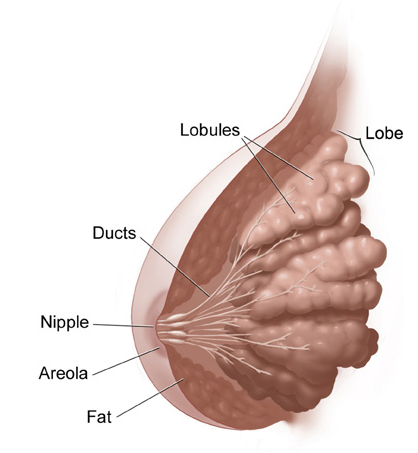
\includegraphics[width = 0.34\textwidth]{plots/breastAnatomy.png}
	\caption[Anatomy of the female breast]{Anatomy of the female breast. Image courtesy of~\cite{NCI2012}.}
	\label{fig:BreastAnatomy}
\end{figure}

The \emph{cancer stage} depends on the size of the tumor and whether the cancer cells have spread to neighboring tissue or other parts of the body. It is expressed as a Roman numeral ranging from 0 through IV; stage I cancer is considered \emph{early-stage breast cancer} and stage IV cancer is considered \emph{advanced}. Stage 0 describes non-invasive breast cancers, also known as \emph{carcinoma in situ}. Stage I, II and III describe invasive breast cancer, i.e., cancer has invaded normal, surrounding breast tissue. Stage IV is used to describe metastatic cancer, i.e., it has spread beyond nearby tissue to other organs of the body.

\subsection{Mammograms}
%\subsubsection{Mammograms}
A \emph{mammogram} is an x-ray image of the breast. Radiologists use \emph{screening mammograms} (normally composed of two mammograms of each breast) to check for breast cancer signs on women who lack symptoms of the disease. If an abnormality is found, a \emph{diagnostic mammogram} is ordered; these are detailed x-ray pictures of the suspicious region~\cite{NCI2014}. A standard mammogram is shown in Figure~\ref{fig:normalMammogram}.

\begin{figure}[h]
	\centering
	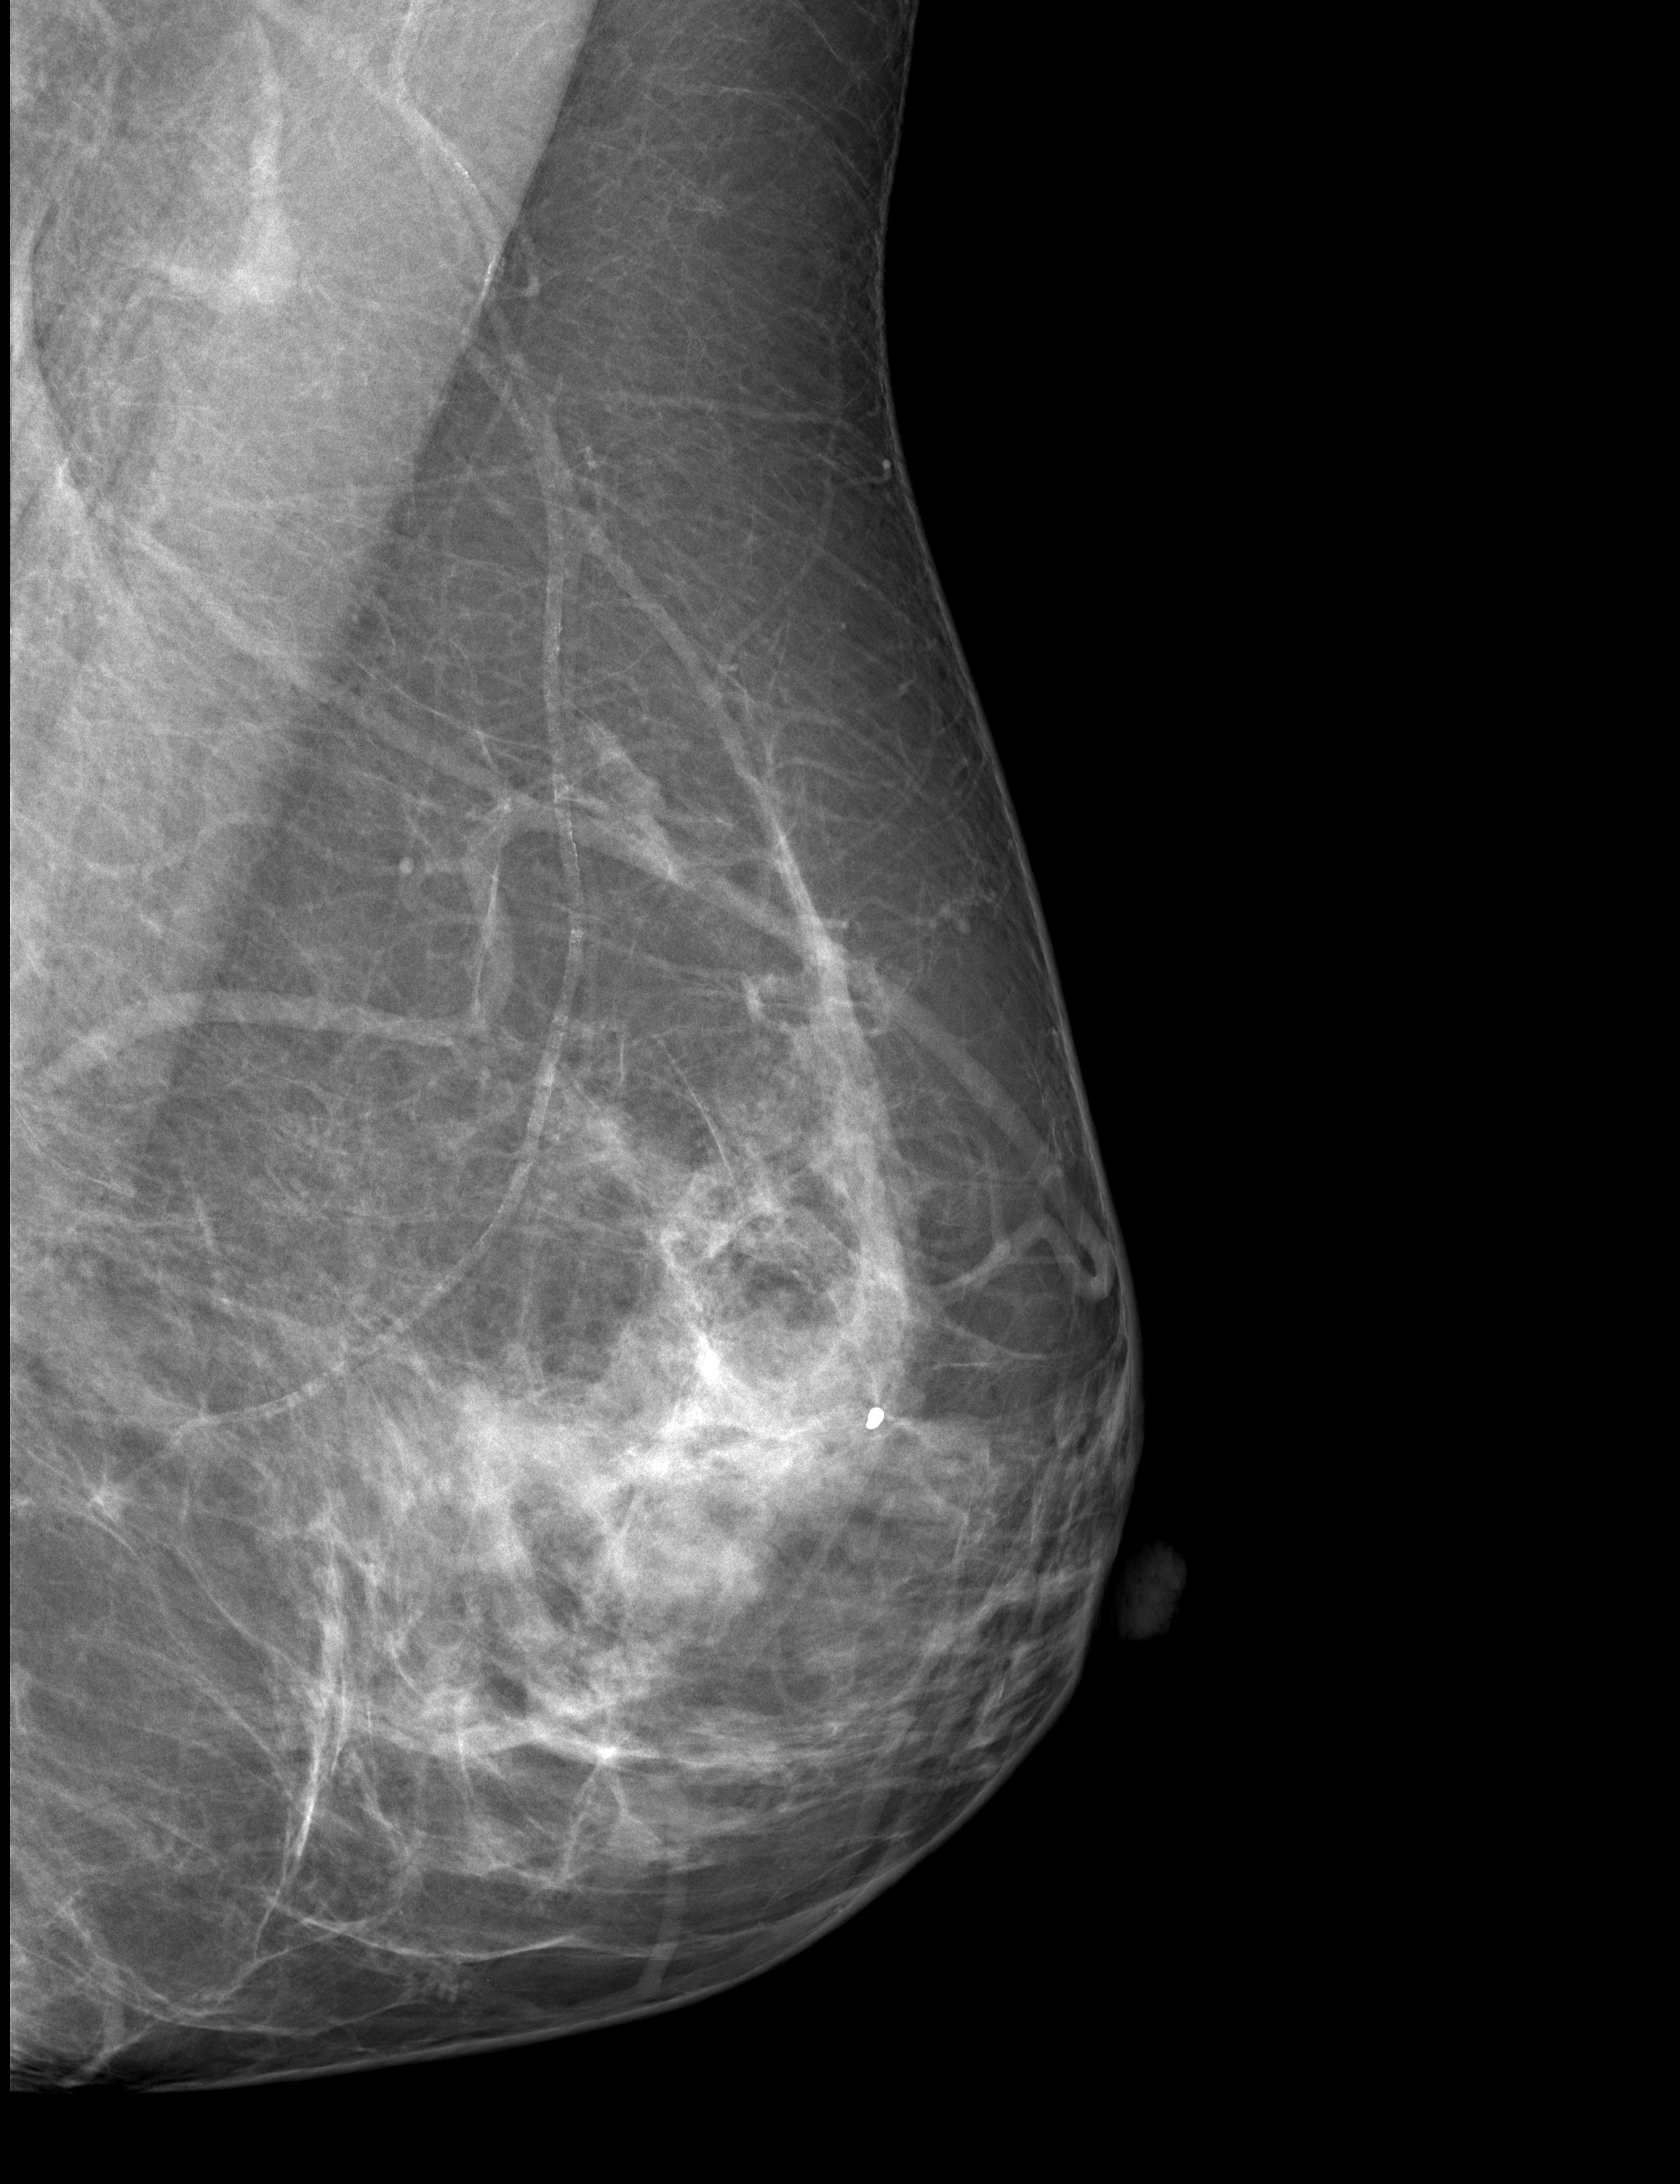
\includegraphics[width = 0.25\textwidth]{plots/normalMammogram.jpg}
	\caption[A digital mammogram]{A standard mammogram.}
	\label{fig:normalMammogram}
\end{figure}

Having a screening mammogram in a regular basis is the most effective method for detecting breast cancer early; around 85\% of breast cancers can be detected in a screening mammogram~\cite{BCSC2013}. Nevertheless, screening mammograms have many limitations: a high false positive rate, overtreatment in Stage 0 cancer, false negative results for women with high breast density, radiation exposure and physical and psychological discomfort~\cite{NCI2014}.

Radiologists look primarily for microcalcifications and breast masses. \emph{Microcalcifications} are tiny deposits of calcium in the breast tissue that can be a sign of early breast cancer if found in clusters with irregular layout and shapes (Fig.~\ref{fig:breastCancerSigns}). \emph{Breast masses} or breast lumps are a variety of things: fluid-filled cysts, fibric tissues, noncancerous or cancerous tumors, among others. A mass can be a sign of breast cancer if it has an irregular shape and poorly defined margins (Fig.~\ref{fig:breastCancerSigns}). Radiologists will also consider the breast density of the patient when reading a mammogram given that high breast density is linked to a higher risk of breast cancer~\cite{ACS2014}.
\begin{comment} My classification
Lesion
	Mass = Lump(This is palpable)
		Malignant = Cancerous
			Tumors
		Benign = Noncancerous
			Tumors
			Cysts
			Fibrosis/Fibroadenoma
	Microcalcifications (benign or malignant)

Tumors are abnormal growths of cells, cysts ae filled with fluid and fibrosis are "firmness in the connective tissues". Lesion is anything suspicious in a mammogram
Detection: Find lesions (malignant or benign)
Diagnosis: Find malignant lesions
\end{comment}

\begin{figure}[h]
	\centering
	\begin{subfigure}{0.24\textwidth}
                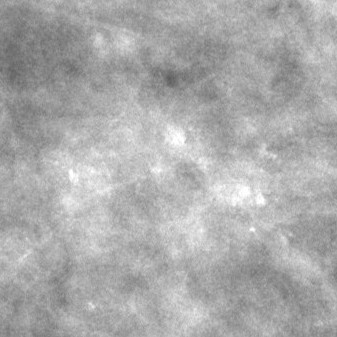
\includegraphics[width=\textwidth]{plots/breastMicrocalcification.jpg}
        \end{subfigure}
	~
	\begin{subfigure}{0.24\textwidth}
                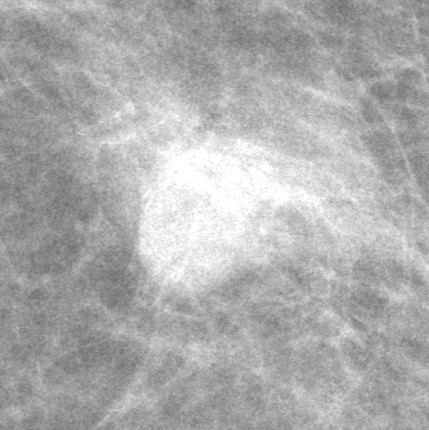
\includegraphics[width=\textwidth]{plots/breastMass.jpg}
        \end{subfigure}
	\caption[Signs of possible breast cancer]{Signs of possible breast cancer in a mammogram. Left: A cluster of microcalcifications in an irregular layout. Right: A poorly defined breast mass.}
	\label{fig:breastCancerSigns}
\end{figure}

%Conventional mammography uses film to record x-ray images of the breast. \emph{Digital mammography}, on the other hand, uses digital receptors that convert x-rays into electrical signals and stores the image electronically. 
Conventional mammography records mammograms in film; \emph{digital mammography}, on the other hand, converts x-rays into electrical signals and stores images electronically.
Digital mammograms offer a clearer picture of the breast and ease manipulation and sharing between health care providers.
% However, researchers still debate whether [[its|their] use over| they] [surpass| improve on|outperform|[offers|have] an advantage over|are more effective than|benefit] film mammograms [in|for] [identifying breast cancer|breast cancer detection].
Although researchers still debate whether they offer an advantage over film mammograms~\cite{Kerlikowske2011, Pisano2008, Skaane2007}, digital mammography has become standard in breast cancer screening. Figure~\ref{fig:normalMammogram} is, in fact, a digital mammogram.

\emph{Digital tomosynthesis} is a new technology that produces three-dimensional x-ray images of the breast and is expected to improve the efficacy of mammograms. Studies comparing the two techniques have not yet been published~\cite{NCI2014}.

\emph{Computer-aided detection (CAD)} systems assist radiologists during screening signaling suspicious areas and displaying relevant information. Detection or CADe looks for any type of lesion while diagnosis or CADx focuses on malignant lesions. Whether their use improves accuracy has been challenged~\cite{Lehman2015}.

% option: Delete this, downgrade mammograms to subsubsection and add the bcdr info in the solution/data set/database part. Maybe also leave the first paragraph in here as part of mammograms subsection, only change it to say "Mammography databases are important"
% option: do not add anything
\subsection{Mammographic databases}
%Databases are essential to mammographic image analysis;
%annotated
Researchers use data from previous patients---mammograms, segmentations and clinical features\textemdash to train and evaluate their models. 
%Databases offer pixel-wise labelled mammograms, lesions are segmented by expert radiologists.
%For this purpose, lesions are manually segmented to produce pixel-wise labels.
\emph{Contrast resolution}, the number of gray values per pixel, and \emph{spatial resolution}, breast area per pixel, dictate the quality of a digital mammogram: 12-bit images ($2^{12} = 4048$ gray values) with pixel size of at most 0.1mm are prefered. Many publicly available databases, including those described below, satisfy these conditions.

The Digital Database for Screening Mammography (DDSM)~\cite{Heath2001} is the most popular database used for CAD development. It is composed of around 10.5K digitized film mammograms from 2620 patients. Mammograms are either 12-bit or 16-bit images with 0.05 mm spatial resolution. Lesion segmentations are provided along with its type, assesment, subtlety and malignancy.%Patient data is also provided.
%Type is mass, microcalcification, assesment (1-5) in BIRADs, subtlety(1-5) and 

The BancoWeb database~\cite{Nepomuceno2011} consists of around 1.5K digitized film mammograms from 300 Brazilian patients. Mammograms are 12-bit images with 0.075 or 0.15 mm pixel size. Although few lesions are segmented, this repository may be useful to assess performance in Latin American patients. Its current state is unknown.

Lastly, the Breast Cancer Digital Repository (BCDR-DM)~\cite{Moura2013a, Moura2013b} consists of around 1.2K digital mammograms from 237 patients. Mammograms are 8-bit images with 0.07mm spatial resolution.
Lesion segmentations are provided as well as their assesment, hand-crafted texture and shape features and relevant clinical data.
%It provides lesion segmentations and assesments, hand-crafted texture and shape features and relevant clinical data

\begin{comment}
Another small digital mammogram repository is called INbreast~\cite{Moreira2012}. It consists of 410 digital mammograms from 115 patients. Each mammogram is a 14-bit image with 0.7 mm spatial resolution. Lesion boundaries are accurately marked and its information is also included. This could be used in conjunction with the BCDR-DM repository.

Finally,~\cite{Zheng2012} used a private repository of around 6.5K digital mammograms obtained from 1120 patients. Specifics of contrast and spatial resolution are not provided but they are most probably good enough. Lesions are marked (with a circle) on the mammograms and lesion and patient information is provided. Even though this is a private repository of the University of Pittsburgh, if needed, we could ask them for access to it. This may not be plausible given the complications of sharing personal (granted anonymized) information and the size of the database.
\end{comment}

This section was written using information from the National Cancer Institute. We recommend to visit its website (\url{www.cancer.gov}) for further details.


	%\subsection{Mammography DB}
	%\label{subsec:MammographyDB}

	\subsection{Classification}
	\label{subsec:Classification}
	%\emph{Machine learning} is the study of algorithms that create models (either of a population or of a function of interest) and estimate their parameters from data  in order to make good predictions or inferences.
%Machine learning is the study of mathematical models either of a population or of a function of interest and the algorithms used to estimate their parameters from data in order to make predictions or inferences.
\emph{Machine learning} is the study of algorithms which build models of a population or a function of interest and estimate their parameters from data in order to make predictions or inferences. A machine learning expert knows how to choose the right model for the problem in hand (\emph{model selection}), how to efficiently estimate its parameters from the available data (\emph{learning} or \emph{training phase}) and how to evaluate the trained model (\emph{testing phase}).

Machine learning problems can be divided into three categories depending on the data used to train the model: \emph{supervised learning}, where we learn a function $f(x)$ using a set of examples which are labelled with the correct output, for instance, learning a function that estimates the price of a house given its size and number of bedrooms from a dataset of houses labelled with their real value; \emph{unsupervised learning}, where we look for relationships and structure in unlabelled data, for instance, given a dataset of potential customers find those who are likely to buy a car and \emph{reinforcement learning}, where the only feedback received are rewards, for example, learning to play tetris from a dataset of world states and actions and where rewards are received sparsely every time points are earned (when lines dissapear). Supervised learning can be further divided in regression and classification. If the expected output is numerical, e.g., the price of a house, it is called \emph{regression}, if the expected ouput is categorical, e.g., spam or no spam, it is called \emph{classification}. We will focus on classification.

A \emph{classifier} takes as input a vector of \emph{features} $x \in \mathbb{R}^n$ from a problem instance and produces an \emph{output} $h(x)$ predicting the class $y$ that instance belongs to, i.e., it concretely models the underlying function $f(x)$ as $h(x)$ ($h$ stands for hypothesis). \emph{Binary classification}, when $y$ can only take two values e.g., cancer/no cancer, is the most common kind of classification and \emph{multiclass classification}, when $y$ can take $K > 2$ different values, can be performed by using $K$ binary classifiers. Some classifiers, such as convolutional networks (defined in Section~\ref{subsec:ConvNets}, output a \emph{score vector} $h(x) \in \mathbb{R}^K$ where $h(x)_k$ is a measure of the probability that $x$ belongs to class $k$. Every classifier partitions the \emph{feature space}, the $n$-dimensional space where features exist, into separate \emph{decision regions}, regions of the space which are assigned the same predicted outcome; a \emph{decision boundary} is the hypersurface that partitions the feature space. Classifiers are sometimes classified as \emph{linear} or \emph{nonlinear} according to the nature of the decision boundary they impose on the feature space. Logistic regression, for instance, is a linear classifier while an artificial neural network (with at least one hidden layer) is nonlinear.
% A linear classifier can separate perfectly linear data, while for nonlinear data a more powerful classifier is needed. Linearly separable data are those which can be classified by a linear classifier while nonlinear data can not.

The \emph{loss function} $J(\theta)$ of a classifier measures the amount of error the classifier incurs in for a particular choice of parameters $\theta$. There are various ways to formulate this function. A \emph{least-squares loss function} for a binary classifier (such as logistic regression) is presented in Equation~\ref{eq:LossFunction}
\begin{equation}
	J(\theta) = \frac{1}{2m}\sum_{i=1}^m(h_\theta(x^{(i)}) - y^{(i)})^2
	\label{eq:LossFunction}
\end{equation}
where $m$ is the number of training examples, $y \in \{0,1\}$ is the real class of the example $x$ and $h_\theta(x) \in \mathbb{R}$ is the output of the classifier for input $x$ with parameters $\theta$, this represents the probability that $x$ belongs to the positive class 1. We introduce another (rather more complex) loss function in the next section.

A classifier is trained by choosing the parameters $\theta$ that minimize its loss function, hence, minimizing the expected error of the classifier on the training set. \emph{Gradient descent} is a method used to estimate the parameters that minimize $J(\theta)$: at the start, it initializes parameters at random and iteratively updates each parameter using the gradient of the loss function until it converges to a minimum. Specifically, at each iteration it performs the update:
\begin{equation}
	\theta = \theta - \alpha \nabla{J(\theta)}
\end{equation}
where $\alpha$, called the \emph{learning rate}, defines the step size. Gradient descent is guaranteed to converge to a global minimum if the loss function is convex, convexity of the loss function depends on the model $h(x)$.

To select the best model $h(x)$ for a particular problem or equivalently to select the best classifier for the problem each model is trained on a subset of the data set and later evaluated on a disjoint subset. In the {validation set approach} the data set is split into a training set (usually 70-90\%) and a validation set, each model is trained using the training set and evaluated on the validation set and the model which shows the best performance is selected. \emph{k-fold cross validation}, on the other hand, divides the data set in $k$ disjoint subsets (usually 5 or 10) and uses $k-1$ subsets to train the model and the remaining subset for evaluation, this process is repeated $k$ times for each model leaving out a different subset each time and the $k$ performance measures are averaged to obtain a final measure for the model.
%Cross validation produces better error estimates but is computationally costly.
\emph{Model hyperparameters}, settings which modify the underlying model or learning algorithm, are selected in the same way.

The model representation $h(x)$ needs to be chosen carefully. If we have an overly \emph{flexible} model, i.e, $h(x)$ is a complex function with many parameters to be learned compared to the size of the training set, the classifier will probably \emph{overfit} the data, this means that the parameters are fitted way too closely to the data and will pick up every small fluctuation and noise in the training set causing the trained classifier to produce almost perfect results on the training set but perform poorly on previously unseen examples. The opposite is also true, when $h(x)$ is very simple the classifier lacks the power to model the function of interest and we say that it \emph{underfits} the data. This problem is sometimes referred as the \emph{bias-variance tradeoff}. A high variance classifier is prone to overfitting, while a high bias classifier is prone to underfitting.

A popular way to avoid overfitting (and underfitting) is to use a flexible model trained with regularization. \emph{Regularization} modifies the loss function to include a penalty to the complexity of the model, thus forcing the learning stage to choose parameters that minimize both the training error of the classifier and the complexity of the model. Equation~\ref{eq:l2NormRegularization} shows the least-squares loss function with \emph{$l_2$-norm regularization}:
\begin{equation}
	J(\theta) =  \frac{1}{2m}\sum_{i=1}^m(h_\theta(x^{(i)}) - y^{(i)})^2 + \frac{\lambda}{2m} ||\theta||_2
	\label{eq:l2NormRegularization}
\end{equation}
where $||\cdot||_2$ is the euclidean norm of a vector. In addition to reducing training error, minimizing the regularized loss function will shrinken the parameters $\theta$ hopefully setting some of them to zero, thus simplifying $h(x)$. The \emph{regularization strength} $\lambda$ regulates the tradeoff between less training error and less regularization error. \emph{$l_1$-norm regularization} or \emph{lasso} is similar to $l_2$-norm regularization except that it shrinks the $l_1$-norm of $\theta$ instead of the $l_2$-norm.

To evaluate the performance of a classifier we use a separate set of examples (a test set) which should have not been used for training or validation. Classification accuracy is the standard performance measure in machine learning. \emph{Accuracy} measures the proportion of test set examples which are correctly classified. Its compliment, \emph{error rate}, measures the proportion of test set examples which are incorrectly classified. Accuracy, nonetheless, is not a good evaluation metric for unbalanced data sets, data sets which have many more examples of one class than the other e.g., cancer data sets are often unbalanced as most examples belong to the negative class (no cancer) than the positive class (cancer). For instance, a classifier which always predicts no cancer regardless of the input will show a high accuracy (equivalently a low error rate) even though it is not a good model for the problem.

A different set of metrics based on the confusion matrix of the classifier are used to evaluate its quality in unbalanced data sets. A \emph{confusion matrix} is a matrix which summarizes the results of a classifier in the test set (see Table~\ref{tab:ConfusionMatrix}).
\begin{table}[h]
	\centering
	\begin{tabular}{cc|c|c|}
		&\multicolumn{3}{c}{\textbf{Actual class}}\\
		&&Positive & Negative \\
		\cline{2-4}
		\textbf{Predicted}&Positive&True Positives (TP)& False Positives (FP)\\
		\cline{2-4}
		\textbf{class}&Negative&False Negatives (FN) & True Negatives (TN)\\
		\cline{2-4}
	\end{tabular}
	\caption{Confusion matrix for a binary classifier}
	\label{tab:ConfusionMatrix}
\end{table}
\emph{True positives} is the number of positive examples which were correctly predicted as positive. \emph{False positives} is the number of negative examples which were incorrectly predicted as positive. True negatives and false negatives are defined in a similar fashion. Based on the confusion matrix we can compute some commonly used metrics:
\begin{equation}
	Sensitivity \text{ or } Recall = \frac{TP}{TP+FN}
\end{equation}
\begin{equation}
	Specificity = \frac{TN}{FP+TN}
\end{equation}
\begin{equation}
	Precision = \frac{TP}{TP+FP}
\end{equation}
Sensitivity and specificity are usually preferred to present results in medical diagnosis meanwhile precision and recall are preferred in machine learning. \emph{Sensitivity} measures the proportion of positive examples predicted as positive and \emph{specificity} measures the proportion of negative examples predicted as negative. \emph{Precision} is a measure of the proportion of examples predicted as positive which are actually positive. A good classifier will have both high sensitivity and high specificity or similarly, high precision and high recall. It is always useful to have a single metric to evaluate classifiers, for example, to choose between two models; we show two commonly used metrics in Equation~\ref{eq:F1Score} and~\ref{eq:G-mean}.
\begin{equation}
	F_1\text{ }score = 2\times\frac{Precision \times Recall}{Precision + Recall}
	\label{eq:F1Score}
\end{equation}
\begin{equation}
	G\text{-}mean = \sqrt{Sensitivity \times Specificity}
	\label{eq:G-mean}
\end{equation}

In this thesis, we will generally present results for all this metrics (precision, recall or sensitivity, specificity, $F_1$ score and G-mean). The metric used when selecting a model influences its characteristics and behaviour, hence, one should put some consideration into choosing it. We favor $F_1$ score over G-mean because it concentrates on prediction in the positive class (cancer) which is harder to predict and the class we are more interested in. Furthermore, it represents a more balanced tradeoff (an small change in precision is corresponded with a small change in recall) than G-mean where an small change in specificity can be corresponded with a big change in sensitivity.
\begin{comment} Discussion of why G-mean over F1
(Not sure about this) As a rule of thumb, using G-mean will generate models that predict more positives given that the sensitivity will greatly improve and specificity will only slightly decrease. Using $F_1$ score, the model will predict less positives as that will improve precision but only slightly decrease sensitivity. 

Why G-means? Because it is more important to obtain a low error in specificity than in precision, i .e, would you prefer a 90% in specificity or a 90% in precision?. 90% in specificity means that 10% of actual negatives (10 persons) were told they have no cancer although they actually had cancer, meanwhile 10% of expected positives(a small number, maybe 1) was said he has cancer although he doesn{t. First is worse.

Using G-mean i will predict more positives, no matter what. My sensitivity is going to vastly improve and the specificity will only decrease a little, but the precision is gonna take a hit. Because if I predict less positives sensitivity is gonna go down, specificity is gonna go up (as I add more true negatives) but just a little and precision  would go up (but it wouldn't matter for g-mean).

Using F1 I'll probably predict less positives, sensitivity is going to go slightly down, and precision is going to go up, specificity doesn{t matter but it will decrease a little. Or I'll probably predcit as many poositives as needed. It focuses more on the positive class.

Other diagonal, the algorithm will learn negatives pretty well, so the one that predicts less positives(f1) probably isn{t learning much (it is predicting all negative).
\end{comment}

This section is meant to be a compendium of basic concepts in machine learning, practical machine learning involves many subtleties and implementation details not mentioned here. Notation and content in this section is mostly based on materials from Stanford's Machine Learning course\cite{Ng2014}.


	\subsection{Artificial Neural Networks}
	\label{subsec:ANNs}
	\emph{Artificial neural networks} or simply \emph{neural networks} are one of the most popular nonlinear classifiers used today. They were initially inspired by the way biological neurons process information coming from its dendrites and relaying it through its axon to neighboring neurons~\cite{McCulloch1943, Widrow1960, Rosenblatt1962} but evolved to become more practical for nonlinear modelling albeit less biologically accurate~\cite{Rumelhart1986}. We discuss here multilayer feedforward neural networks, the name should become obvious after a few paragraphs.

\emph{Multilayer feedforward neural networks} are composed of $L$ layers of \emph{neurons}, units of computation, each of which is fully connected to the next and previous layer (except for the first and last layer). The first layer, called the \emph{input layer}, has $s^{(1)} = n$ units and receives the feature vector $x \in \mathbb{R}^n$ meanwhile the last layer or \emph{output layer} has $s^{(L)} = K$ units corresponding to the $K$ possible classes. Every other layer is called a \emph{hidden layer} (see Fig.~\ref{fig:NeuralNetwork} for an example). The neural network receives an input $x \in \mathbb{R}^n$, processes it layer by layer and outputs a vector $h_\Theta(x) \in \mathbb{R}^K$, where $h_\Theta(x)_k$ is the predicted (unnormalized log) probability that $x$ belongs to class $k$. Each unit performs a computation on the input from the units in the previous layer and transmits the result to the units in the next layer through its connections. Furthermore, each connection has a \emph{weight} $w$ which is to be learned in the training phase, i.e, the weights are the parameters $\Theta$ of the model. A neural network is said to be \emph{shallow} or \emph{deep} according to its number of layers or \emph{depth}.\footnote{There is no consensus on when a neural network becomes a deep neural network\cite{Schmidhuber2015}. We consider networks with over 2 hidden layers to be deep.}

\begin{figure}[h]
	\centering
	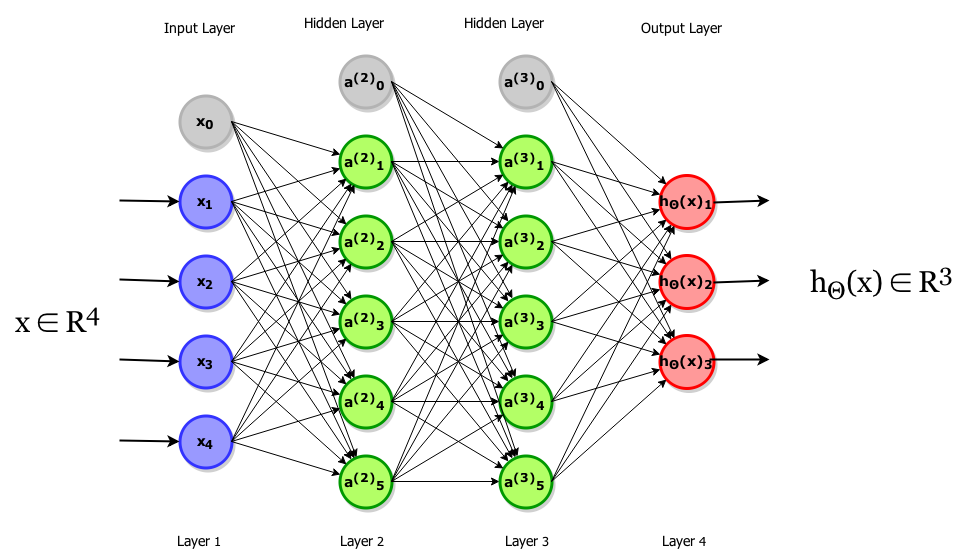
\includegraphics[width = \textwidth]{plots/neuralNetwork.png}
	\caption[Example of an Artificial Neural Network]{Small neural network example. Input layer with 4 units (blue), two hidden layers of 5 units (green) and output layer of 3 units(red). Bias units appear in gray. It approximates a function $h_\Theta(x): \mathbb{R}^4 \to \mathbb{R}^3$, i.e., it classifies an input vector $x \in \mathbb{R}^4$ into 3 possible classes.}
	\label{fig:NeuralNetwork}
\end{figure}

A unit $i$ in layer $l$ computes a function of the form:
\begin{equation}
	a^{(l)}_i = g \left(\sum_{j=0}^{s^{(l-1)}} \Theta^{(l-1)}_{ij}a_j^{(l-1)}\right) \text{ for $l= 2,\dots,L-1$ and $i = 1,\dots,s^{(l)}$}
	\label{eq:NeuronActivation}
\end{equation}
where $a^{(l)}_i$ is called the \emph{activation} or output of unit $i$ in layer $l$;
$g(\cdot)$ is an \emph{activation function} (defined below);
$s^{(l)}$ is the number of units in layer $l$;
$a^{(u)}_0 = 1$, for all $u = 1, \ldots, L-1$ (bias units);
$a^{(1)}_v = x_v$ for all $v = 1, \ldots, n$ i.e, the activation of the input layer is the input $x$;
$a^{(L)}_i = \sum_{j=0}^{s^{(L-1)}} \Theta^{(L-1)}_{ij}a_j^{(L-1)}$ for all $i = 1,\dots,s^{(L)}$ i.e, $g(\cdot)$ is not applied in the output layer
and $\Theta^{(l)} \in \mathbb{R}^{s^{l+1} \times s^{l}} $ is the matrix of weights connecting layer $l$ to $l+1$. At each layer (except the output layer) we include a unit which always emits activation 1 ($a^{(1)}_0 = 1$, $a^{(2)}_0 = 1$, etc), these are called \emph{bias units}~
\footnote{They are included for a technical detail: so that the activation function $g(w^Tx+w_0)$ can shift in the x-axis changing its threshold to $-w_0$, which is learned by the neural network.}. 
The bias units are assumed to be included into each vector $a^{(l)}$, hence the sumation in Equation~\ref{eq:NeuronActivation} starts at 0 and not 1. It may seem like a convoluted definition but it simply defines the activation of a given unit as the weighted linear combination of activations of the units in the previous layer passed through a nonlinear function $g(\cdot)$.
Lastly, notice that $a^{(L)} \in \mathbb{R}^{s^{(L)}}$, the vector of activations in the last layer of the network, is equal to the predicted (unnormalized log) probabilities $h_\Theta(x) \in \mathbb{R}^K$, also called a \emph{score vector}. The class with the highest score in $h_\Theta(x)$ is the predicted class for the example $x$. We could also exponentiate each of these probabilities and normalize them to obtain a distribution of probabilities over the possible classes $K$ ($p(x) \in [0..1]^K$). This improves interpretability but does not change the predicted classes.

\begin{comment}
The activation function $g(\cdot)$ is usually a \emph{logistic sigmoid function}:
\begin{equation}
	g(z) = \frac{1}{1+ e^{-z}}
\end{equation}
The sigmoid function has range [0,1] and is differentiable with respect to $z$. Because of this characteristics it is used to represent probabilities in the logistic regression classifier. \emph{Logistic regression} for binary classification models the probability that $x \in \mathbb{R}^n$ belongs to the positive class as $g(w^Tx)$ and estimates the parameters $w \in \mathbb{R}^n$ during training. Any input whose output $g(w^Tx)$ is greater than $0.5$ is classified as positive, otherwise it is classified as negative. The sigmoid function equals $0.5$ when $w^Tx = 0$, thus, the decision boundary of a logistic regression classifier is $w^Tx = 0$, which is a linear function. 

However, the sigmoid function, per se, is not linear on its input $z$. Therefore, each unit in a neural network with sigmoid activation functions outputs a nonlinear activation $g(z)$ which in turn is received by units in the next layer, linearly recombined with the activation of other units and passed again through a sigmoid function; these operations are repeated until the input reaches the output layer. As a result, the function calculated by units in the output layer $h_\Theta(x)$ will be highly nonlinear on the original input $x$. This is the reason why neural networks can model functions which are highly nonlinear and why increasing the number of layers in a neural network increases the predictive power of the model. By the same token, it may be insightful to think of each unit in a neural network as a feature detector (via logistic regression): units in the first hidden layer are trained to activate when simple features are found on the input, units on the second hidden layer activate when a combination of these simple features is present on the input and so on. Thus, the network will learn to detect the most relevant features for the classification task and as the number of units increases, it learns ever more complex features (granted that there is enough training data).
\end{comment}

The activation function $g(\cdot)$ is usually a \emph{rectified linear unit} or \emph{ReLU}:
\begin{equation}
	g(z) = \max(0,z)
\end{equation}
This is a nonlinear activation function which is very easy to implement in numerical computations, its derivative ($1_{z>0}$) can be calculated quickly and does not suffer from vanishing or exploding gradients as do the sigmoid or tanh activation functions. Furthermore, it has been shown to greatly accelerate the convergence of gradient descent~\cite{Krizhevsky2012}. For these reasons it is the currently recommended activation function for deep neural networks~\cite{Karpathy2015}.

Each unit in a neural network outputs a nonlinear activation $g(z)$ which in turn is received by units in the next layer, linearly recombined with the activation of other units and passed again through a nonlinear function; these operations are repeated until the input reaches the output layer. As a result, the function calculated by units in the output layer $h_\Theta(x)$ will be highly nonlinear on the original input $x$. This is the reason why neural networks can model functions which are highly nonlinear and why increasing the number of layers in a neural network increases the predictive power of the model. By the same token, it may be insightful to think of each unit in a neural network as a feature detector: units in the first hidden layer are trained to activate when simple features are found on the input, units on the second hidden layer activate when a combination of those simple features is present on the input and so on. Thus, the network will learn to detect the most relevant features for the classification task and as the number of units increases, it learns ever more complex features (as long as there is enough training data).

The \emph{softmax} cost function for a multiclass neural network classifier is defined as:
\begin{equation}
	J(\Theta) = -\frac{1}{m} \sum_{i=1}^m \log \left ( \frac{ e^{h_\Theta(x^{(i)})_{y^{(i)}}} }{ \sum_{j=1}^K e^{ h_\Theta (x^{(i)})_j} } \right )
\end{equation}
where $m$ is the number of examples in the training set, $h_\Theta(x)$ is the score vector, $K$ is the number of classes and $(x^{(i)},y^{(i)})$ is the $i^{th}$ example. $J(\Theta)$ is differentiable with respect to $\Theta$ but non-convex, nonetheless, gradient descent usually converges to a good estimate of the network weights~\cite{Ng2014}. \emph{Error backpropagation}~\cite{Linnainmaa1970, Werbos1974}, an algorithm to calculate the derivatives with respect to $\Theta$ needed for gradient descent, computes the error terms in the output layer and backpropagates them layer by layer using the chain rule of derivatives. Given the big number of parameters which need to be estimated, neural networks are susceptible to overfitting. The simplest approach to overcome this problenm is to use regularization. Regularization for neural networks is done by performing gradient descent on the regularized cost function presented in Equation~\ref{eq:ANNRegularizedCostFunction}
\begin{equation}
	J(\Theta) = -\frac{1}{m} \sum_{i=1}^m \log \left ( \frac{ e^{h_\Theta(x^{(i)})_{y^{(i)}}} }{ \sum_{j=1}^K e^{ h_\Theta (x^{(i)})_j} } \right ) + \frac{\lambda}{2m}\sum_{l=1}^{L-1}\sum_{i=1}^{s^{(l)}}\sum_{j=1}^{s^{(l+1)}} \left(\Theta^{(l)}_{ij}\right)^2
	\label{eq:ANNRegularizedCostFunction}
\end{equation}


	\subsection{Convolutional Networks}
	\label{subsec:ConvNets}
	\emph{Convolutional networks}, also \emph{ConvNets} or \emph{CNNs}, were first inspired on the way the human visual cortex proccesses information~\cite{Fukushima1980} but, as regular neural networks, they have evolved to favor practical performance over biological accuracy. LeCun et al. used a convolutional network to achieve good classification performance on the MNIST data set of handwritten digits~\cite{LeCun1989, LeCun1998}, the first successful application of modern convolutional networks. Recently, they have been used to achieve state-of-the-art performance on the ImageNet Large Scale Visual Recognition Challenge~\cite{Krizhevsky2012}, an image classification and object localization challenge with 1000 categories~\cite{Russakovsky2014}. Since then, thanks to various advances (maxpooling , ReLU activations, weight initialization, GPU training, efficient backpropagation, etc.) they have become one of the most popular methods for image classification tasks and (along with recursive neural networks for generative models) an emblem for deep learning.

In this section we show the standard features and training of current convolutional networks, Section~\ref{subsec:PracticalDL} gives some practical advice for choosing hyperparameters and training deep architectures. For an in depth review of convolutional networks, see \cite{Karpathy2015}. For a complete overview of the history and state of deep learning, see \cite{Schmidhuber2015}.

Convolutional networks map raw image pixels to a score vector $h_\Theta(x) \in \mathbb{R}^K$ representing the distribution of (unnormalized log) probabilities over the $K$ classes. We could easily use a regular neural network (presented in Section~\ref{subsec:ANNs}) to do this classification but the amount of learnable parameters (the weights) becomes very big. For instance, a small color image of size $100\times100$ with 3 color channels (RGB) will require $30\,000$ units in the input layer and each unit in the second layer will therefore have $30\,000$ weights to learn. This is impractical not only because it will require a lot of data and time to train but because the loss function has very many local minima and thus it is harder to find a good local minimum.

Convolutional networks are specially designed to handle images reducing the number of connections between layers and the number of parameters to learn. Instead of fully connected layers such as regular neural networks convolutional layers are \emph{sparsely connected}, i.e., a unit is only connected to a small subset of the units in the previous layer. Furthermore, they are \emph{locally connected}, i.e., units are connected considering their position on the original image. The architecture of a convolutional network also imposes \emph{weight sharing} between layers, i.e., different connections are forced to share the same weights (this determines filters and feature maps, defined below). \emph{Pooling} is a subsampling mechanism that reduces the spatial scale and makes the computations invariant to local translation. All this features reduce computation and improve the classification performance of convolutional networks; they are a product of the way convolutional networks are defined, which we explain below.

Each layer is composed of a set of \emph{feature maps}, 2-dimensional grids of unit activations~($\mathbb{R}^{h\times w}$), arranged into a 3-dimensional matrix ($\mathbb{R}^{h\times w \times d}$) where the third dimension is used to put together all feature maps. One could think of each layer as having all unit activations in a single column as in regular neural networks but seeing them as a 3-dimensional volume makes the definitions easier. The input layer could be considered as a 3-dimensional matrix ($\mathbb{R}^{h\times w \times c}$) holding the image of size $w\times h$ with $c$ color channels (usually one for grayscale images or three for RGB). The output layer could also be thought of as a volume of size $R^{1\times 1 \times K}$ where each feature map is just one activation ($R^{1\times 1}$) representing the final score. The convolutional network then receives an input image $x$, transforms it into the first layer of feature maps (which does not need to have the same dimensions as the previous layer) and keeps transforming it until we have an output layer of size $h(x) = R^{1\times 1 \times K}$. See Fig.~\ref{fig:ConvNetVolumes} for an illustration. We describe the possible transformations next.
\begin{figure}[h]
	\centering
	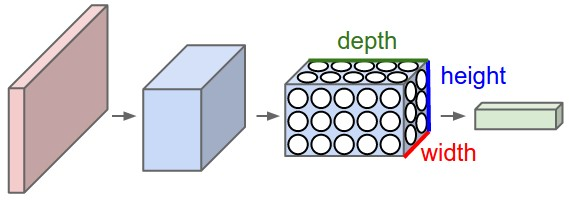
\includegraphics[width = 0.7\textwidth]{plots/convNetVolumes.jpeg}
	\caption[Convolutional network visualization]{A simple representation of the transformations of the input that a convolutional network computes. Input layer is shown in pink, hidden layers are shown in blue and output layer is shown in green. The third layer has 5 feature maps of size $2\times3$. Notice that the width is listed first by convention. Image courtesy of~\cite{Karpathy2015}.}
	\label{fig:ConvNetVolumes}
\end{figure}

There are four types of layers: convolutional layer, ReLU layer, pooling layer and fully connected layer all of which compute a differentiable function on its input and combine to form a convolutional network architecture.

\paragraph{Convolutional layer} Convolutional layers are the heart of convolutional networks. They are composed of a set of learnable filters which will be applied to the volume in the previous layer. A \emph{filter} is a matrix of weights 
which has a small spatial size (width and height) but goes across all feature maps of the volume (the third dimension). For instance, a $3\times 3$ filter to be applied in a volume with 10 feature maps will have 90 parameters ($\mathbb{R}^{3\times3\times10}$). See Figure~\ref{fig:ConvLayer} for an example. Each feature map in this layer is obtained by sliding a filter across the spatial dimensions (width and height) of the previous volume computing the dot product (a weighted sum) between the filter and the input producing a 2-dimensional array of values~\footnote{Each filter has also a bias term which is added to the product.}. Notice that all values in a single feature map are computed using the same filter. If we think of the feature map as a grid of units we can see that every unit is connected with only a small local subset of the units in the previous layer and that all units in the map share the same weights. 

At each convolutional layer, many feature maps are computed (each with its own filter) and stacked together to form the volume in the layer. We can think of each filter as looking for an specific feature of the input and each feature map collecting the probabilities of the feature being present in different positions of the original image.

We need to define various hyperparameters for this layer: the filter size, the stride (the number of places to shift the filter at each step), the amount of zero padding around the image and the number of feature maps. These define the shape of the resulting volume; the first three are usually defined in a way that it preserves the spatial size of the previous volume, the third dimension is solely dependent on the number of feature maps desired.
\begin{figure}[h]
	\centering
	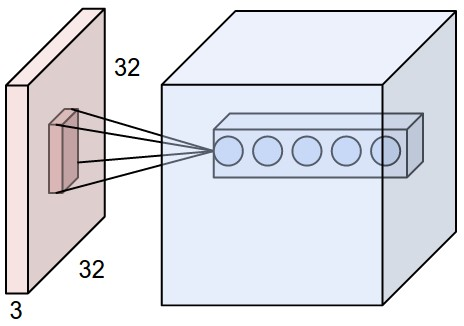
\includegraphics[width = 0.4\textwidth]{plots/convLayer.jpeg}
	\caption[Example of a filter in a convolutional layer]{Example of a filter applied to a volume ($\mathbb{R}^{32\times 32\times 3}$) to obtain the values shown in the blue volume. The filter comprises all 3 feature maps of the input volume. We compute 5 feature maps as shown by the 5 units in the blue volume. For a complete convolution this filter will have to slide across the input volume. Notice all units in the same feature map share the same filter but units in different feature maps do not, even though they can be connected to the same local region of the input. Image courtesy of~\cite{Karpathy2015}.}
	\label{fig:ConvLayer}
\end{figure}

\paragraph{ReLU layer} This layer receives an input volume and performs an elementwise ReLU activation function to it, i.e, each value $z$ in the volume is passed through the nonlinearity $\max(0,z)$. It does not change the dimensions of the volume and has no learnable parameters, although the activation function itself could be considered as a hyperparameter. Usually a convolutional layer is always followed by a ReLU layer (or any other activation function), for this reason they are sometimes considered part of the convolutional layer, we leave them separate for clarity.

\paragraph{Pooling layer} The pooling layer subsamples the volume on the spatial dimensions reducing the size of the feature maps but keeping the number fixed. Standard max pooling slides a fixed size windows (normally $2\times2$) along each feature map with stride 2 (it is, without overlapping) and selects the maximum element on that space. This will reduce each dimension of the feature map by half, thus reducing the total number of activations by 75\%, e.g., a $4\times4$ feature map gets subsampled to size $2\times 2$ where each value is the maximum activation on each of the four quadrants of the original feature map. Notice that the subsampling is applied to each feature map separately contrary to the convolution. A popular variant of max pooling uses $3\times 3$ windows with stride 2, allowing for overlapping in the pooling.

\paragraph{Fully connected layer} One or more fully connected layers are used at the end of the network to compute the final score vector. Feature maps in this layer have size $1 \times 1$ resulting in a row volume or alternatively a row vector of values. Each feature map in this layer is fully connected to all units in the previous volume and outputs a dot product between the input and the connection weights which are the parameters to be learned during training. The output layer of a convolutional network is always a fully connected network with as many feature maps as classes. The interpretation of the scores of the output layer is similar to that of regular neural networks as the (unnormalized log) probability of $x$ belonging to class $k$. Lastly, notice that a fully connected layer can be simulated by a convolutional layer with the same number of feature maps and filter size $w\times h$ where $w$ and $h$ are the dimensions of the feature maps in the previous layer, i.e, filters that comprise the entire previous volume.

\bigskip
Convolutional layers (plus ReLUs) compute features on the input while pooling layers shrinken the volume before passing to the fully connected layers which act as a neural network classifier on the obtained features. The standard convolutional network architecture can be represented textually as:
\begin{verbatim}
       INPUT -> [[CONV -> RELU]*N -> POOL?]*M -> [FC -> RELU]*K -> FC
\end{verbatim}
where \texttt{*N} indicates that the layers are repeated \texttt{N} times, \texttt{?} indicates that the layer is optional and \texttt{N,M,K >= 0}. We can use this template to construct ever more flexible models from a linear classifier \texttt{INPUT -> FC} (\texttt{N,M,K = 0}) to a regular neural network \texttt{INPUT -> [FC -> RELU]+ -> FC} (\texttt{N,M = 0}, \texttt{K > 0}) to a convolutional network \texttt{INPUT -> [[CONV -> RELU]+ -> POOL?]+ -> [FC -> RELU]* -> FC} (\texttt{N,M > 0}, \texttt{K >= 0}). For instance, a typical deep convolutional network could be:
\begin{verbatim}
        INPUT -> [[CONV -> RELU]*2 -> POOL]*3 -> [FC -> RELU]*2 -> FC
\end{verbatim}
This network receives an input volume (the image) computes two sets of convolution plus ReLUs before pooling and repeats this pattern three times followed by fully connected layers plus ReLUs which are repeated twice and the output layer which reports the final classification scores. Although there is no standard way of counting the number of layers of a convolutional network usually the ReLU or pooling layers are not counted as they have no learnable parameters, therefore our example architecture has 10 layers (21 in total) which is a good depth for big data sets. Practical recommendations on building convolutional network architectures is offered in the Section~\ref{subsec:PracticalDL}.

% Counting layers (?)

Figure~\ref{fig:ConvNetExample} shows an example of a convolutional network with its different kind of layers. The image is taken from a simulation accesible at \url{cs231n.stanford.edu}.

\begin{figure}[h]
	\centering
	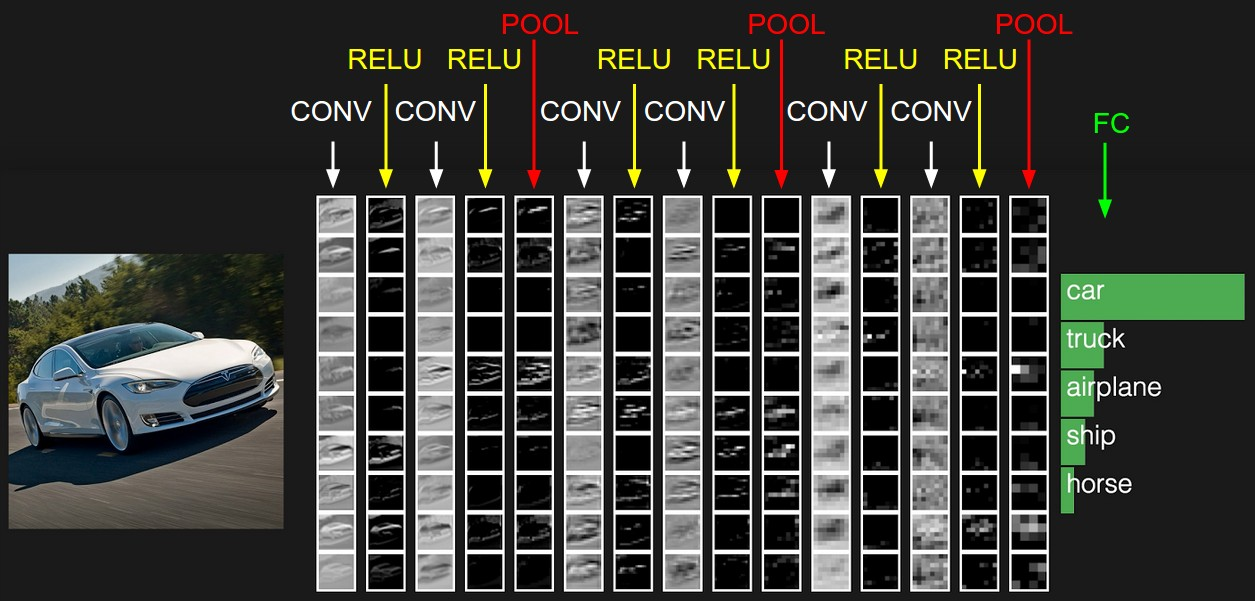
\includegraphics[width = 0.85\textwidth]{plots/convNetExample.jpeg}
	\caption[Example of a convolutional network in action]{Example of a convolutional network with architecture \texttt{INPUT -> [[CONV -> RELU]*2 -> POOL]*3 -> FC}. The input image has size $32\times 32$. Each hidden layer uses 10 feature maps (shown as columns). Notice that although the size of the feature maps looks constant in fact each pooling layer reduces each dimension by half (the feature maps of the final pooling layer have size $4\times 4$). The final scores are shown only for the 5 most probable classes. Image courtesy of~\cite{Karpathy2015}.}
	\label{fig:ConvNetExample}
\end{figure}

Recently there has been a push towards simpler convolutional network architectures. The All Convolutional Net~\cite{Springenberg2014} is a network formed solely by convolutional layers: pooling layers are replaced by convolutional layers with larger strides and fully connected layers are replaced as explained above. Notice that this greatly increases the number of parameters to be learn, therefore it may not be suitable for small data sets.

Converting the fully connected layers to convolutional layers has another advantage: we can use a convolutional network trained on small images to classify bigger images. By the way convolutional layers are defined when a bigger image is used as input the entire convolutional network will slide across the image and be applied to different portions of the image generating a score vector for each of them. Therefore, instead of having a single score for each class we will have an entire matrix of scores (for each position where the convolutional network was applied). We can then average over all scores per class to obtain a single score vector for the bigger image. Furthermore, we can control the stride of the convolution to choose how the convolutional network is slided across the big image.
For instance, if we train a convolutional network with images of size $32\times 32$ which via pooling get reduced to feature maps of size $4\times 4$ in turn passed to the (converted) fully connected layers to obtain a score vector, then when using a $96\times 96$ image as input to the same convolutional network it will get reduced to feature maps of size $12 \times 12$ and the fully connected layers will output a matrix of scores of size $9\times 9$ (for each class), i.e, it slides the $4\times 4$ fully connected layers across the $12\times 12$ feature maps. Averaging each score matrix we obtain the final scores for the big image. We could have also  set a stride of 4 in the first (converted) fully connected layer to get score matrices of size $3\times 3$ for each 9 non-overlapping $32\times 32$ partitions of the original image. It works exactly as if we were applying the convolutional network to the original image at a stride of 32 but does all computations in just one pass. This way we can reuse a pretrained network to classify images of bigger size. 

\emph{Transfer learning} is a related method where a convolutional network is trained on images from a specific domain and later used as a feature extractor for images on a different domain or as a initialized network which is fine tuned with examples of the new domain.

The loss function for a multiclass convolutional neural network is similar to that for a regular neural network (Equation~\ref{eq:ANNRegularizedLossFunction}) except that the vector score $h_\Theta(x)$ is now defined by the architecture of the convolutional network.
\begin{equation}
	J(\Theta) = -\frac{1}{m} \sum_{i=1}^m \log \left ( \frac{ e^{h_\Theta(x^{(i)})_{y^{(i)}}} }{ \sum_{j=1}^K e^{ h_\Theta (x^{(i)})_j} } \right ) + \frac{\lambda}{2m}\sum_{l=1}^{L-1}\sum_{i=1}^{s^{(l)}}\sum_{j=1}^{s^{(l+1)}} \left(\Theta^{(l)}_{ij}\right)^2
	\label{eq:ConvNetLossFunction}
\end{equation}
Furthermore, this loss function is still differentiable with respect to $\Theta$ and thus the entire network can be trained via gradient descent. Gradients of the loss function are also calculated using backpropagation.


	\subsection{Convolutional Networks applied to Breast Cancer}
	\label{subsec:BreastCancerConvNets}
	Yet to write. Redacted version of section Related Work.

	\subsubsection{Related Work}
	%\label{subsubsec:RelatedWork}
	In this section we offer a summary of some of the first work on using convolutional networks for breast cancer diagnosis as well as some of the articles that have influenced this thesis.

Lo et al.\cite{Lo1995} were the first group to use convolutional networks for breast cancer detection. They used a CNN with two hidden layers to detect microcalcifications. A high sensitivity image processing technique was used to obtain a set of 2104 patches (16 by 16 pixels) of all potential disease areas from 68 digital mammograms; of these, 265 were true microcalcifications and 1821 were ``false subtle microcalcifications". Prior to training the CNN, a wavelet high-pass filtering technique was used to remove the background of these images. Each image was flipped over (left-right) and 4 rotations for each the original and flipped images were used for training (0°, 90°, 180° and 270°). The CNN was composed of one input unit ($16\times16$), 12 units in the first hidden layer ($12\times12$), 12 units in the second hidden layer($8\times 8$) and two output nodes(one for YES and one for NOT). The input size ($16\time16$), number of hidden layers ($2$) and kernel size ($5\times5$) was obtained via cross validation, altough not many other options were explored: they tried input sizes of 8, 16 or 32, one or two hidden layers and kernel sizes of 2, 3, 5 or 13. The CNN reached 0.87 average AUC when identifying individual microcalcifications and 0.97 AUC for clustered microcalcifications. Only a minimum of three calcifications was considered a detection. Sensitivity and specificity test results were not reported. This article proved that simple convolutional networks can be efficiently used for medical image pattern recognition.
%Lesson learned: two hidden layer newtwork produces better results, background reduction is neccesary and using matrices invariance to augment the data helps. Convnets work helps and convnets work.

%A refined approach was presented some years later by the same authors along some non convolutional neural networks~\cite{Lo1998}. The setting is very similar but ..... Results are..

%work done at Tec


	\subsection{Practical Deep Learning}
	\label{subsec:PracticalDL}
	In this section we collect guidelines for building as well as efficiently training deep convolutional networks; while they are specific to this thesis, they may prove useful in similar projects. Deep learning is a fast-changing field so these recommendations may soon outdate.
% Some of these details are taken care by the software(either as a defualt or optional feature) and some are qyuite new and need to be taken care manually. 

\paragraph{Image preprocessing} Convolutional networks handle raw image data, but some level of preprocessing speeds training and improves performance.
\begin{itemize}
	\item Crop images to contain only the relevant regions, denoise, enhance and resize them to maintain the input size fixed and manageable.

	\item Zero-center each image feature (the raw pixels) by subtracting its mean across all training images. Optionally, normalize each zero-centered feature to range from $[-1 \dots 1]$ by dividing them by its standard deviation~\cite{Karpathy2015}.

	\item Test data should not be used to calculate any statistic used for preprocessing. Furthermore, the same statistics (calculated from training data) should be used to preprocess test data~\cite{Karpathy2015}.
\end{itemize}



\paragraph{Convolutional network architecture} Designing convolutional networks involves many decisions, we provide recommendations for the architecture and sensible values for related hyperparameters.

\begin{itemize}
	\item Select a network architecture flexible enough to model the data and manage overfitting rather than a simpler architecture that may be incapable to model the data~\cite{Ng2014, Krizhevsky2012}. 

	\item Although, theoretically, neural networks with a single hidden layer are universal approximators provided they have enough units ($\mathcal{O}(2^n)$ where $n$ is the size of the input), practically, deeper architectures produce better results using less units overall. This holds for convolutional networks~\cite{Bengio2014}.

	\item Use at least 8 layers (not counting pooling or ReLU layers) for big data sets, use less layers or transfer learning for small data sets. ``You should use as big of a neural network as your computational budget allows, and use other regularization techniques to control overfitting.''~\cite{Karpathy2015}

	\item Use 2-3 \texttt{CONV -> RELU} pairs before pooling (N above)~\cite{Karpathy2015}. Pooling is a destructive operation, placing two convolutional layers together allows them to detect more complex features.

	\item Use 1-5 \texttt{[CONV -> RELU]+ -> POOL} blocks (M above). This hyperparameter regulates the representational power of the architecture. The exact number depends on the complexity of the features in the data and the computational resources available. It also defines how much the volume is subsampled.

	\item Use less than 3 \texttt{FC -> RELU} pairs before the output layer (K above)~\cite{Karpathy2015}. The volume that arrives to fully connected layers is already complex, adding many layers only increases the number of parameters and risks overfitting.

	\item The number of feature maps per convolutional layer controls the number of features detected at that layer---similar to the number of units per layer in a regular neural network. A common pattern is to start with a small amount of feature maps and increase them layer by layer~\cite{Simonyan2014}. %The reasoning is that at higher layers there are more complex features to learn and moreover as the feature maps become smaller (via pooling) it is computationally feasible to have more of them.

	\item The number of feature maps per fully connected layer decreases layer by layer\footnote{The number of units in a convolutional layer is the number of units in a feature map times the number of feature maps.}. For instance, for a convolutional network with ten possible classes and two fully connected layers, if the last convolutional layer produces a volume of size $8 \times 8 \times 512$ (8192 units), the first fully connected layer could have size $1 \times 1 \times 2048$ and the second--- the output---layer $1\times 1\times 10$.

	\item Use $3\times 3$ filters with stride 1 and zero-padding 1 or $5 \times 5$ filters with stride 1 and zero-padding 2. This preserves the spatial dimensions of the volume and works better in practice~\cite{Springenberg2014}. If the input size is too big, use a bigger filter in the first convolutional layer~\cite{Karpathy2015}.
	
	\item Use $2\times2$ pooling with stride 2. This pooling and the overlapping version presented in Section~\ref{sec:ConvNets} produce similar results~\cite{Krizhevsky2012}.
%krizhevsky says overlapping is slightly better. so does dieleman but it slows thing down.
	\item Use square input images (width = height) with spatial dimensions divisible by 2. These should be divisible by 2 at least as many times as the number of pooling layers in the network.

	\item Use number of parameters to measure the complexity of an architecture rather than number of layers or units.
\end{itemize}



\paragraph{Hyperparameters} About setting and searching hyperparameters other than those of the network architecture.

\begin{itemize}
	\item Use a single sufficiently large validation set (15-30\% of data) rather than cross validation~\cite{Bengio2014}. Use cross validation in very small data sets~\cite{Ng2014}.

	\item Use random search rather than grid search. Random search draws each parameter from a value distribution rather than from a set of predefined values.~\cite{Bergstra2012}

	\item Search for the best combination of hyperparameters rather than each individually.

	\item Train each combination of hyperparameters for 1-2 epochs to narrow the search space; then, train for more epochs on these ranges~\cite{Karpathy2015}. Explore further when the best value for a hyperparameter is found in the limit of the range.~\cite{Bengio2012}.

	\item Partial convergence is sufficient to assess hyperparameters~\cite{Karpathy2015}.

	\item Hyperparameters related to the convolutional architecture, e.g., number of layers, number of feature maps and filter sizes are set manually (as explained above) rather than using a validation set.

	\item Several hyperparameters are set: initial learning rate $\alpha$, learning rate decay schedule, regularization strength $\lambda$, momentum $\mu$, probability of keeping a unit active in dropout $p$, mini-batch size and type of image preprocessing.

	\item We could fit all hyperparameters using a validation set but, in practice, this is computationally unfeasible and results in overfitting to the validation data~\cite{Cawley2010}.

	\item Set $\alpha$, $\lambda$ and optionally the type of preprocessing using a validation set. Other hyperparameters can be set to a sensible default. 
%The learning rate schedule and training epochs are set using heuristics. 

	\item The learning rate $\alpha$ is ``the single most important hyperparameter and one should always make sure that it has been tuned''~\cite{Bengio2012}. It ranges from $10^{-6}$ to $10^{0}$. Use a log scale to draw new values ($\alpha = 10^{unif(-6, 0)}$ where $unif(a,b)$ is the continous uniform distribution)~\cite{Karpathy2015}.
%0.01: Bengio, 2012 says that the optimal learning rate is close to the highest learning rate that does not cause divergence.

	\item The regularization strength $\lambda$ is usually data (and loss function) dependant. It ranges from $10^{-3}$ to $10^4$. Search in log scale ($\lambda = 10^{unif(-3, 4)}$).
%1
	\item Halve the learning rate every time the validation error stops improving or choose a fixed number of epochs by observing when the validation error stops decreasing in a similar network~\cite{Krizhevsky2012}.

	\item Use $\mu=0.9$. If using a validation set try values in \{0.5, 0.9, 0.95, 0.99\}~\cite{Karpathy2015}.

	\item Use 0.9-1 probability $p$ of retaining a unit in the input layer, 0.65-0.85 in the first 2-4 convolutional layers and 0.5 in the last convolutional layers and all fully connected layers~\cite{Srivastava2014}. Less dropout is used on the first layers because they have less parameters~\cite{Karpathy2015}.
% Maybe don't use dropout in the input layer, because putting a zero there has a meaning(black), maybe the advantage of dropout in cinvolutional layers is just that it adds noise to the input.

	\item Use mini-batch size of 64 or 32. A larger batch size requires more memory and training time. Test performance is unaffected~\cite{Bengio2012}.

	\item Choose among standard preprocessing techniques by (qualitatively) inspecting results on images from the validation set. If none seems superior, fit it along $\alpha$ and $\lambda$% other hyperparameters.
\end{itemize}



\paragraph{Training} Convolutional networks have millions of parameters and require careful training. We offer general advice and list some commonly used techniques.

\begin{itemize}
	\item Shuffle training examples before each epoch to ensure that examples in every mini-batch are sampled independently~\cite{Bengio2012}.

	\item Multiply the number of examples by 25-100 to estimate the maximum number of parameters that could be learned (assuming data augmentation). Groups have learned up to 40M parameters from as little as 60K training examples~\cite{Dieleman2015, Springenberg2014}.

	\item Weight initialization is vital for convergence. Initialize each filter weight as a value from a normal distribution $\mathcal{N}(\mu = 0, \sigma = \sqrt{2/n_{in}})$ where $n_{in}$ is the number of connections to the filter (9 for a $3\times 3$ filter)~\cite{He2015}. In code, \texttt{w = randn()*sqrt(2/nIn)} where \texttt{randn()} returns values drawn from a standard normal distribution. Initialize biases likewise.

	\item Use mini-batches rather than the entire training set to compute the gradient of the loss function. Mini-batches allows us to make more updates, more frequently resulting in faster convergence and better test results~\cite{Bengio2012}.

	\item Use Nesterov's Accelerated Gradient (NAG) to update the weights. NAG is a modified version of gradient descent that works better for certain architectures~\cite{Bengio2012b}. Stochastic Gradient Descent with Momentum (SGD+Momentum) is also a viable option~\cite{Karpathy2015}.
% May need to crossvalidate the momentum if using NAG 

	\item Use dropout as a complement to $l_2$-norm regularization. Dropout improves results but may slow network convergence~\cite{Krizhevsky2012}.

	\item Store network parameters regularly during training. This allows us to inspect the network at different stages, retrain one or select the one with the best validation error~\cite{Bengio2014}.
	%\item Use the validation or test error to select the best parameters for the network from those stored~\cite{Bengio2014}. 

	\item Stop training if the validation error has not improved since the last learning rate reduction: gradient descent may not have converged but the validation error will start to increase (overfit)~\cite{Bengio2012}.

	\item If you used test set results to refine a model, shuffle the entire data set and choose a different training and test set to avoid overfitting to the test set~\cite{Ng2014}.
\end{itemize}


\paragraph{Sanity checks}
We perform some simple tests to make sure training works properly.
\begin{itemize}
	\item After weight initialization, run a test on a small set of examples to assert that the network predicts similar scores for every class, the loss function without regularization equals $-\log(1/K)$ and adding regularization increases the loss~\cite{Karpathy2015}.

	\item Run a gradient check if backpropagation seems faulty. Gradient checks compare the analytic gradient obtained via backpropagation with a numerical gradient obtained via a finite difference approximation~\cite{Karpathy2015}.

	\item Train the network (without regularization) in 10-40 examples to check that the loss function becomes zero. If the network is unable to overfit a tiny subset of data, flexibilize the model.~\cite{Ng2014}.

	\item During training, the loss function evaluated on training examples decreases monotonically~\footnote{Because of momentum and regularization it could also increase slightly before decreasing.}. If not, check for implementation errors, reduce the learning rate or augment momentum~\cite{Karpathy2015}.

	\item Monitor the loss function during training to identify underfitting, characterized by high training loss and high validation loss, and overfiting, characterized by low training loss and high validation loss~\cite{Ng2014}.
\end{itemize}

\paragraph{Image segmentation} We usually require to post-process, upsample and threshold the output of a convolutional network to produce a valid segmentation. 
Given that the network is already trained, using the validation set to choose the best techniques is virtually free.% Here we account for some details about this additional steps.

\begin{itemize}

	\item For big input images, use smaller mini-batches to avoid overloading the GPU memory~\cite{Karpathy2015}.

	\item Set the post-processing technique using the validation set. Conditional random fields are specially effective for refining convolutional network scores~\cite{Chen2015}.

	\item Use bilinear interpolation for upsampling~\cite{Chen2015}. If the upsampling factor is greater than 16, use a learnable upsampling layer or skip layers~\cite{Long2015}.

	\item Set the segmentation threshold using the validation set; this hyperparameter is equivalent to the threshold used in classification.

\end{itemize}

\paragraph{Data augmentation} We reduce overfitting in image data by applying label-preserving transformations to the original images to generate additional examples. Transformations include rotations, translations, horizontal and vertical reflections, crops, zooms and jittering (adding noise to the colors).  The network receives different views of the object and learns invariant features; for instance, if we present images of books at different rotations, we expect it to learn to identify a book on any orientation.
% Dieleman galaxies didn't like jittering or scales and crops
% Lo liked rotation and horizontal flipping

\begin{itemize}
	\item Exploit invariances you expect in the data set, e.g., galaxies are rotation-invariant because in space there is no up or down~\cite{Dieleman2015}.% but trees are not as we rarely see an upside down tree.

	\item Be careful to preserve the original label of the image. Applying many transformations may cause the image to lose its meaning. 

	\item Generate the augmented images during training to save storage~\cite{Krizhevsky2012}.

	\item If applying many affine transformations, combine them into a single operation. This is faster and reduces information loss~\cite{Dieleman2015}.

	\item Optionally, use data augmentation at test time: present the network with different versions of the image and average its predictions~\cite{Krizhevsky2012}.
\end{itemize}

% Need some sources for this section. I've read it all around.
\paragraph{Unbalanced data}
In practice, it is common to have very few examples of one class compared to the rest. Managing unbalanced data sets is still an open problem.%We offer advice to deal with unbalanced classes.using standard convolutional networks.
\begin{itemize}
	\item For binary classification with rare positive class, use PRAUC as a performance metric. If the threshold is selected using a validation set, $F_1$ score is also valid~\cite{Davis2006}.

	\item For multiclass classification, use the macro-averaged $F_1$ score, an average of $F_1$ scores per class, with validated thresholds~\cite{Ozgur2005}. A multiclass PRAUC exists but is not used.

	\item If using an appropiate metric is impractical, divide each predicted class probability by the prior probability of the class and renormalize~\cite{Bishop1995}. This rescales predictions to account for the original imbalance in the class distribution.

	\item Avoid oversampling, repeating examples from the rare class, and undersampling, discarding examples from the dominant class, because they do not add any information to the data set.

	\item If rare examples are insufficient for learning, augment them more or balance each mini-batch via stratified sampling; the latter is oversampling.%data replication (oversampling).% Augmentation differs from replication in that it enriches the data set with invariant images but proportion of classes remains unchanged.

%	\item One of the preferred methods to learn with unbalanced data sets is to use a modified loss function which gives a higher weight to errors in the rare class so that during training errors in the rare class will produce higher learning in the network parameters. Specific knowledge of the domain is required to estimate the cost of each class of error.
\end{itemize}

\begin{comment}
\paragraph{All convolutional networks}
The research community has been moving towards discarding pooling layers and using all convolutional networks; interpreted as letting the network learn the pooling operation. We offer a couple of guidelines for implementing all convolutional networks.  
\begin{itemize}
	\item Replace each pooling layer with a convolutional layer with as many feature maps as the previous layer and filter size $2\times 2$ with stride $2$ for normal pooling or $3\times 3$ with stride $2$ for overlapping pooling~\cite{Springenberg2014}. 

	\item For small data sets pooling layers also work as a regularizer because they reduce the number of learnable parameters and replacing them with convolutional layers may not be convenient~\cite{Karpathy2015}.
\end{itemize}

\paragraph{Transfer learning}
When we have a small data set we could use a pretrained convolutional network either as a feature extractor for the new examples or to provide initializations for the new convolutional network, this is called transfer learning. We offer some tips for using a pretrained model specifically for mammographic images.

\begin{itemize}
	\item Using a convolutional network pretrained in natural images, such as the ImageNet database, CIFAR-10, CIFAR-100, etc., may not work for mammographic images because features useful for one kind of classification are not very useful for the other. Nonetheless, given that features become more specific at higher layers, we could discard the higher layers of the network and use only the cropped network~\cite{Karpathy2015}.
 
	\item Depending on the amount of data that we have we could: (1) add some fully connected layers on top of the pretrained network and train only these new layers, (2) add some convoutional and fully connected layers and train these new layers or (3) add convolutional and/or fully connected layers and train the entire network~\cite{Karpathy2015}.

	\item When training on a pretrained model or fine-tuning use an smaller learning rate than when training a network from scratch. Using a small learning rate assures that we do not disturb very much the already good network parameters.~\cite{Karpathy2015}.
\end{itemize}
\end{comment}

\paragraph{Software} We shortly describe four of the most popular packages for deep learning. All have similar capabilities and are available to the public (open-source).

\begin{itemize}
	\item Tensorflow~\cite{Abadi2015} is a Python/C++ library released by Google that supports automatic differentiation on data flow graphs---neural networks, included---, training on clusters of CPUs and GPUs, graph visualization and easy deployment in multiple platforms. It has been quickly adopted by the deep learning community.
	\item Caffe~\cite{Jia2014}: Caffe is a mature deep learning framework developed in C++/CUDA by the Berkeley Vision and Learning Center (BVLC) and community contributors. It offers a Python, Matlab and command line interface; reference models and tutorials; and very fast code with easy GPU activation.
	\item Theano~\cite{Bergstra2010, Bastien2012}: Theano is a Python library developed in Python/CUDA at the University of Montreal. It is tightly integrated with NumPy, performs symbolic automatic differentiation and uses the GPU to efficiently evaluate mathematical expressions involving multidimensional arrays.
	\item Torch7~\cite{Collobert2011}: Torch is a scientific computing framework developed in C/Lua/CUDA at the IDIAP Research Institute. It offers multidimensional arrays (tensors), automatic differentiation, a command line and Lua interface, GPU support and easy building of complex neural network architectures.
%	\item Cuda-ConvNet2~\cite{Krizhevsky2014}: Cuda-ConvNet2 is a highly optimized convolutional network library developed in C++/CUDA by Alex Krizhevsky. It offers different off-the-shelf configurations for convolutional networks, a command line interface and multi-GPU training.
\end{itemize}

\bigskip

We acknowledge that mammographic data is different from regular image segmentation data: labelling is imperfect, image sizes and ratio change, images are bigger, quality varies, objects of interest are small in relation to the background, data sets are smaller, texture is uniform across the image, among others. Therefore, some of the advice given above may prove counterproductive. Whenever possible, design decisions should be based on data and compiled results.
%Deep Learning (Bengio Lecture): (https://www.youtube.com/watch?v=JuimBuvEWBg)


\section{Methodology}
\label{sec:Methodology}
In order to achieve the proposed objectives and test our hypotheses we will need to carry out various tasks. We list them here in the order in which we plan to execute them: %although some steps could be executed simultaneously:

\begin{itemize}
	\item Literature review: A thorough review of the published work using the databases and resources available in the institution. By the end of this task, a complete theoretical background should be obtained and written. This will also help refine the scope of the project and the experiments to be conducted.
	\item Software review: Once a clear idea of what are the possible experiments to be executed, we will need to find appropiate software to perform them. Software for database managing, preprocessing and implementation of different neural networks should be either located or developed.
	\item Database preprocessing: We will ready the database images for the experiments; these implies joining different databases, obtaining the required features, preprocessing the images, assigning labels, etc.
	\item Assesing image preprocessing: We will train a standard convolutional network with fixed parameters on mammograms with three different preprocessings: no preprocessing, image enhancement using median or gaussian filters and wavelet filtered images. Furthermore, we will train a deeper convolutional network on nonpreprocessed images. We want to answer three research questions: which is the best preprocessing for convolutional networks, is using the best filter significantly better than using nonpreprocessed images and can a convolutional network automatically preprocess the images?
% Q: Is it better to make different preprocessings oin the same convolutional network or to fit each convolutional network for each preprocessing, thus, giving it the best chance to perform but taking more time.
	\item Exploratory experiments: We will train standard convolutional networks in two different inputs: small image patches obtained from mammograms and whole mammogram images. We will also train a linear classifier, probably rectified linear units, on the features obtained from a convolutional network trained on the ImageNet database, i.e., we will use an already trained convolutional network instead of one trained specifically in mammograms. Here we will use the image preprocessing technique that showed better results in the previous step. We want to answer two research questions: Can a convolutional network trained on whole mammograms perform as well as one trained on small patches and can we use an already trained convolutional network to classify mammograms?
	\item Model selection: Using the insights from previous sections and the current literature on convolutional networks, we will select a network architecture along with novel features, preprocessing, training and regularization procedures. We aspire to find the best convolutional network configuration for mammogram classification.
	\item Further experimentation: We will train the chosen convolutional network on our mammographic database. We will perform crossvalidation to adjust the most important network parameters and use regularization to avoid possible overfitting. We want to answer two research questions: is the performance of the convolutional network considerably improved by parameter tuning and, more importantly, is this a good performance?.
%Maybe train one with no tune fitting.
	\item Gathering results: Produce results on the test set and elaborate figures and tables. This could be obtained directly from software output or from further program executions.
	\item Reporting results: Write the thesis and any article or technical guide which may result from this work. Both this and the previous step will be performed along the execution of the project, hopefully benefiting from the supervisors' feedback.
\end{itemize}
Finally, we want to note that this is an idealized workflow and some changes may occur due to time limitations or resources unavailability. In the unlikely case that the work is finished before the project deadline, we will either reiterate on model selection, experiments, result gathering and reporting or look into digital tomosynthesis, network ensembles or evolving convolutional networks.

\begin{comment}
La {\it Metodología} (o lo que algunos autores llaman el {\it Método})
 es el proceso o
conjunto de pasos que debe efectuarse para llegar a cumplir con los
objetivos. Esos pasos deben contener  los experimentos a realizar, la forma de
llevarlos a cabo, la evaluación de los resultados, la prueba de las hipótesis,
la respuesta a las preguntas de investigación y el último paso debe ser el
reporte escrito de los resultados.
\end{comment}


\section{Work Plan}
\label{sec:WorkPlan}
Yet to write

\begin{comment}
Una vez establecida la {\it Metodología} es importante establecer las
actividades con sus tiempos respectivos en lo que se llama el {\it Plan de
Trabajo}. Ello nos da una idea clara de la extensión en tiempo del trabajo
propuesto. Además de ser necesario, lo cual es normalmente cierto en
propuestas de proyecto industrial, es importante establecer el PLAN FINANCIERO
el cual desglosa los recursos necesarios para el desarrollo del proyecto y sus
costos.

{\bf Un ejemplo de Plan de Trabajo}

La figura \ref{ttphd} presenta el cronograma de las actividades que llevarán a
cabo los objetivos de esta tesis. 

\begin{figure}[th]
	\centerline{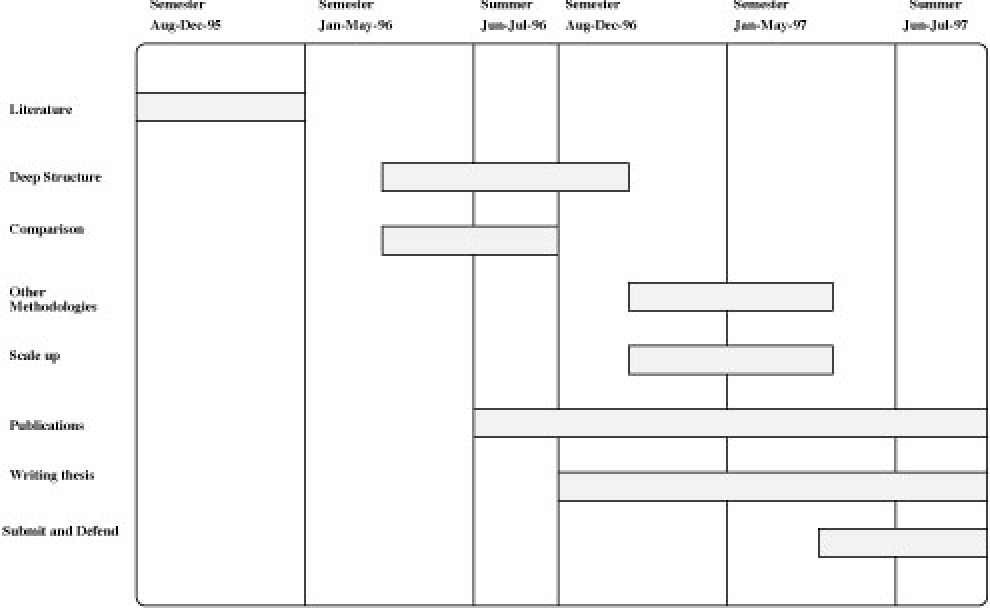
\includegraphics[width=4in,height=3in]{plots/ttphd.pdf}}
	\caption{Cronograma de Actividades para desarrollar la Tesis}
	\label{ttphd}
\end{figure}
\end{comment}


% Bibliography
\bibliographystyle{apalike}
\bibliography{bibliography}

\end{document} 
